\documentclass[twocolumn,12pt]{article}
\usepackage[utf8]{inputenc}
\usepackage{amssymb}
\usepackage{graphicx}% Include figure files
\usepackage{dcolumn}% Align table columns on decimal point
\usepackage{bm}% bold math
\usepackage{subcaption}
\usepackage[sorting=none]{biblatex}
\addbibresource{biblio.bib}
\usepackage{amsmath}
\usepackage{esint}
\usepackage{systeme}
\usepackage{algorithm2e}
\usepackage{blindtext}
\usepackage{subcaption}
\usepackage{minted}
\usepackage{stackengine}
\usepackage[a4paper,margin=0.5in]{geometry}
\title{\textbf{Photovoltaic System Reconfiguration strategy for mismatch conditions}}%\\
           %\emph{Application to mixed typed of data in lung Adenocarcinoma subtype discovery}}
\date{July 2018}
\author{\textbf{Dafang Zhao}\\Nara Institute of Science and Technology, Dependable System Lab}

\begin{document}
\maketitle

\section{Introduction}
\\As the world of fossil energy constantly exhausted and the increasingly serious environmental pollution, the research and utilization of renewable energy and green energy have become maintain necessary means of survival and development of the human. Photovoltaic (PV) energy received significant attention since it has unlimited energy and easy to be scaled up. Thanks to extensive technology and research on photovoltaic energy generation, large scale photovoltaic energy generation system have been deployed into many practical application. But PV arrays are senstive to shading and PV cell's fault or aging. That means the interconnection of PV cells or modules which do not have identical properties or which experience different conditions from one another.
\section{Related work}
\subsection{Lung adenocarcinoma papers}

Here, we will mainly discuss 3 previous works about LUAD and some work on Maximum Likelihood clustering techniques.
Starting with the work of Hayes et al.\cite{hayes}, whom put in evidence from DNA microarrays data, a total cohort of 231 LUAD patients and 2,553 reliable genes, the presence of 3 clusters.
These clusters were found using consensus clustering\cite{cons}, the genes used came from centroids comparison and gene enrichment analysis.
Although this study focused on survival rates, which is not our case, it managed to find strong evidences concerning the existence of three distinct LUAD subtypes named Bronchoid, Magnoid and Squamoid having different gene expression profiles and clinical relevance. \cite{hayes} also managed to identify sets of genes strongly related to each found subtypes, these genes will be taken in consideration in our study.
The second important study is Wilkerson et al.\cite{wilk}, aimed to have a better understanding of the LUAD molecular pathogenesis in order to find better targets for chemo-treatments.
The study focused on DNA alteration, DNA methylation and mutation occuring in LUAD.
They also used cohort wise centroids and ConsensusClusterPlus\cite{consensusPlus} for a total of 462 patients (GSE data set).
They confirmed the clinical differences between the molecular subtypes, showing that the survival rate and therapy response was differing according to each subtype.
The last study we will discuss is the one from TCGA\cite{TCGA}.
This study mainly focused on the relation between the morphological classification and the gene expression profiles, renaming the 3 known subtypes as Proximal-Inflammatory (PI, former Squamoid), Proximal-proliferative (PP, former Magnoid)and Terminal Respiratory Unit (TRU, forner Bronchoid).
They used RNA-seq data as well, data that we will use in our study (TCGA data set), 230 patients and 22k+ genes.
They used RNA-seq data to study mutations in LUAD and they compared their results of subtype detection with \cite{wilk}, finding high correlation between respective clusters.

\subsection{Hierarchical Maximum Likelihood algorithms}

We want to present here some existing methods, implementing a maximum likelihood approach. Note that our desire is to implement a fully Bayesian approach, which differs slightly, furthermore we have to deal with different categories of data.
Castro et al.\cite{castro}, described two different algorithms for clustering purpose using maximum likelihood estimation and MCMC chains. The first algorithm, called Agglomerative Likelihood Tree (ALT), looks for the Maximum Likelihood Tree (MLT) after computing a measure of similarity based on maximum likelihood estimates paiwise.
The MLT obtained by this algorithm will be binary structured.
The second algorithm, called MLT estimator, takes a more global approach.
Searching directly for the MLT in the tree's forest, it allows non-binary association in trees and smartly uses the ALT algorithm to reduce the space of research. 
Both models aren't adapted to mixed type data, which means a generalisation should be implemented.
Sharma et al.\cite{sharma}, implemented a new algorithm for clustering purpose (called HML), their algorithm is able to deal with the Small Sample Size problem, occurring when the covariance matrix in small sample size and high dimension (which is the case with gene expression profiles), using a Singular-Value Decomposition (SVD) method.
Although HML gave promising results, the SVD approach should be trade out in order to deal with categorical data, applying Multiple Factor Analysis (MFA)\cite{pages} decomposition method for instance.
We also can cite an interesting paper concerning hierarchical clustering algorithm by D.Müllner\cite{mullner}, which served as inspiration for our own algorithm creation.

\subsection{Bayesian inference related papers}

We will see later that our method considers the Bayes factor to cluster our data or appreciate a given clustering solution, our reference in that regard is the paper of E.Raftery\cite{raftery}, giving a comprehensive approach to it.
The book \emph{Pattern Recognition And Machine Learning}\cite{bishop}, provided us useful insights to Bayesian inference and related techniques.
Finally, an analytically tractable solution in our Gaussian marginal likelihood with conjugate prior theoritical model, we used an unpublished paper from Kevin P.Murphy\cite{murphy}.

\section{Methods}
\subsection{Data pre-processing}\label{sec:preprocess}

Because we are working with 2 different data sets, it is important to take care of the gene annotation. Indeed, the data set GSE\cite{shedden} is annotated with probe names where the TCGA\cite{TCGA} is annotated with gene symbols (HGNC).
The first step is to use different annotation tables and databases available on R (AnnotationDbi)\cite{annot}, and from the sources of the data sets in order to obtain comparable data sets.
After manipulation of different gene annotations, a gene set in TCGA's data were discarded due to the absence of correspondence in the databases (additional file 1). We also only kept the genes that are in common between GSE and TCGA data sets, discarding the others (Additional file 2) for comparison purpose.
Concerning clinical data, The TCGA data set gives us access to a lot of clinical information, but in order to keep a relevant comparing ground with GSE and also to simplify the study we chose to keep only 4 clinical variables (Sex, Age, Race, Smoking history).
Clinical data were arranged by convenience, the "Age" variable was divided in 8 categories according to the distribution frequencies, and "smoking history" was changed to match its description from the GDC data portal concerning clinical data:
\begin{enumerate}
    \item : Lifelong non-smoker
    \item : Current smoker
    \item : Current reformed smoker $>$ 15 years
    \item : Current reformed smoker $\leq$ 15 years
    \item : Current reformed smoker duration unknown
    \item : Smoker at diagnosis
    \item : Unknown
\end{enumerate}

Because the available clinical data for GSE does not make any distinction between categories 3 and 4, we considered them as category 5, the 7\textsuperscript{th} category was considered as missing value (NA under R software).

Among the genes between our two data sets, we decided to explore different gene sets, and study their ability to differentiate molecular sub-types. Indeed, if we can show satisfying results using only a relevant subset of genes it could simplify analyses and diagnosis of new patients.
Hence we considered two gene sets, one containing the genes described in \cite{hayes} but also the centroids of \cite{wilk} and the 100 most mutated genes in LUAD (GDC data portal) which we called "predictors" gene set. The second one is based on a deferentially expressed genes analysis (DEG) using the R package \emph{DEGseq}.
As we had access to the raw count of transcripts from RNA-seq for TCGA, we were able to perform a DEG analysis.
\begin{figure}[th]
    \centering
    \begin{subfigure}[t]{0.20\textwidth}
        \centering
        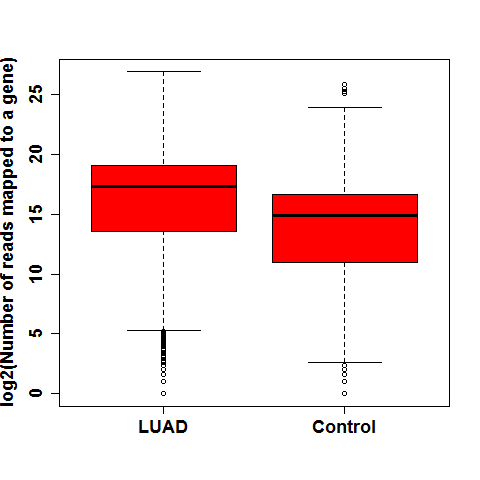
\includegraphics[height=1.6in]{img/SampleS_box.png}
        \caption{Box plots of diseased patients and healthy ones}
        \label{fig:my_label}
    \end{subfigure}
    \begin{subfigure}[t]{0.20\textwidth}
        \centering
        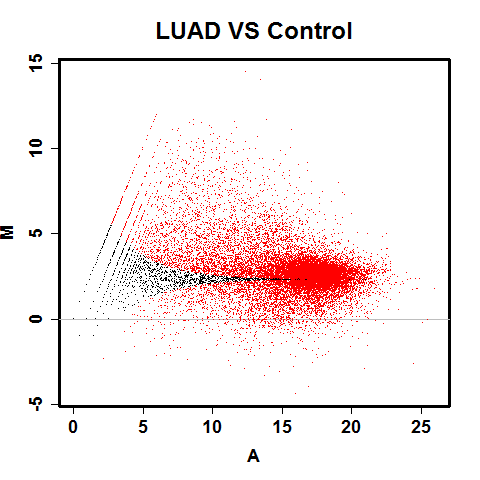
\includegraphics[height=1.6in]{img/result.png}
        \caption{MA-plot of diseased patients and healthy ones (controls)\\
        red dots represent DEG}
        \label{fig:my_label}
    \end{subfigure}
    \caption{DEG analysis using DEGseq package}
    \label{fig:my_label}
\end{figure}
We also compared each sub-type to our controls, taking the sub-type classification given by the TCGA study\cite{TCGA}, see additional file 3.
Each sub-type showed more than 17000 DEG, but in order to stay on the same scale as the predictors gene set and also to keep the ability to differentiate between at least 3 sub-types, we kept only the DEG unique to each sub-type, obtaining a 2000+ genes gene set with only one gene in common with the predictors gene set, which was discarded.
Finally, and for the following analyses, we split our two data sets into four distinct ones:
\begin{table}[!]
    \centering
    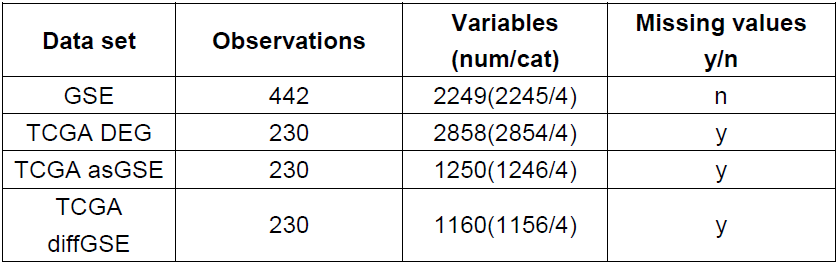
\includegraphics[scale=0.4]{img/adenodatasets.png}
    \caption{Lung Adenocarcinoma data sets}
    \label{tab:adeDt}
\end{table}
In table~\ref{tab:adeDt}, only the "predictors" gene set is kept for the GSE data set because the DEG analysis was performed on the raw counts of the TCGA data set.
Because of some differences in the annotations, the presence of alias in HGNC annotation and absence of some of them in the databases used, the "predictors" gene set gave two possibilities for the TCGA data set, "AsGSE" has exactly the same genes as in GSE, but "diffGSE" gets about a hundred genes different with the GSE data set.

\subsection{Hierarchical clustering}

Clustering analysis has been and still remains an important tool in machine learning oriented research. Clustering methods are not statistical analyses, indeed, the simple fact of clustering
does not grant a final and unique solution. Actually, clustering data randomly will just regroup these data into clusters, but it does not mean that these clusters will have a real meaning, hence our desire to provide here a method assessing this problem and providing statistical significance to clustering results.
Finding the number of clusters (K) that reflects the true classes in the data is an important challenge and can determine the quality of the results. 
Concerning health care purposes, the quality and accuracy of the result represents a great deal, a life saving one.
Indeed, the ability to rightly find cancer sub-types allow researchers and physicians to better adapt to each patient particular case, and find new efficient drugs.
Thus, we developed a Bayesian model comparison method for this purpose.
Our method will be detailed later on, for now lets discuss quickly a certain type of clustering algorithm, and the kind of data we worked on.
The data sets we wish to cluster are comprised of different types of data, indeed, the gene expression profiles (GEP) are of numerical continuous type, where clinical knowledge is of categorical type. By categorical type, we mean variables taking a certain range of values (categories) but lacking a mathematical meaning, having or not an order.
Numerical data can be discrete or continuous, here no problem to understand the continuous form of GEP, on the other hand, categorical data types need some explanations.
There are several types of categorical data in our definition of it:
\begin{itemize}
    \item Binary: A variable which can take only two possible values, i.e: Gender (M/F)
    \item Nominal: Generalisation of the binary case for K categories, i.e: Race (Australoid/Capoid/Caucasoid/Mongoloid/Negroid)
    \item Ordinal: As nominal but with an order, i.e: Age
    \item Interval: similar to ordinal but considering intervals between the values, i.e: also Age
\end{itemize}
It is important to differentiate these data types because the mathematical tools we apply to them are different, their treatment will also be different.
Numerical variables, in our case, will be normalised (log2, $\frac{x-\mu}{\sigma}$...), and categorical ones will be conveniently transformed from characters (MALE/FEMALE), to numbers (1/2), even though it is not absolutely necessary.
When it will come to the Bayesian treatment, numerical variables will be assumed to follow Gaussian distributions (close to a Gaussian distribution when we look at the histogram), and categorical ones multinomial distributions, which change completely their handling.
Our focus in this study is the hierarchical approach of clustering, thus, we give here further information about this popular clustering method with R.
\begin{figure}
    \centering
    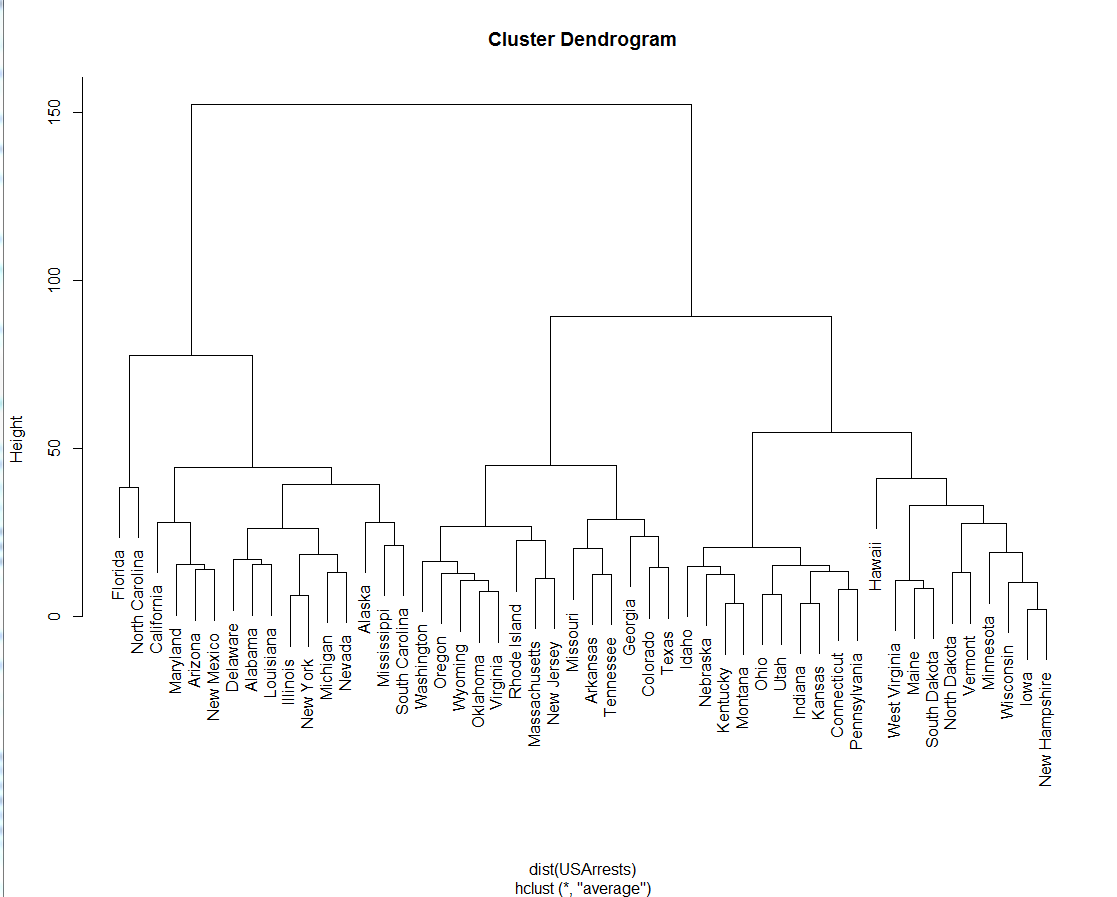
\includegraphics[scale=0.2]{img/HC.png}
    \caption{Example of Hierarchical Clustering with R.}
    \label{fig:HC}
\end{figure}
Hierarchical clustering algorithms are a well documented type of algorithm and rely on similarity/dissimilarity matrix produced by distance metrics in order to pair in an agglomerative manner each samples of a given data set.
Furthermore, the hierarchical scheme get along nicely with the Bayesian model comparison method.
A very simple distance metric example would be the Euclidean distance, defined as:\\
$$d(i,j)\ =\ \sqrt{\sum_{d=1}^D(j_d-i_d)^2}$$


where i and j are two samples of a data set of dimension D.
The choice of the metric is primordial and has to reflect the data types and needs of the user, in our case, and because we have both numerical and categorical types, we decided to use the Gower distance:\\
$d(i,j)\ =\ \frac{1}{N}\sum_{n=1}^Nd_{ij}^{(d)}$\\


Where i and j two samples, N the total number of samples in the data set.\\
$d_{ij}^{(d)}$ is given by:\\
$$d_{ij}^{(d)}\ =\ \frac{|x_{id}-x_{jd}|}{R_d}$$


Where $x_{id}\ \text{and}\ x_{jd}$ are the value of the samples i and j for the variable $d$.
$R_d$ is the range for the variable $d$, dividing by the range avoid to give more weight to variables with greater range.
The Gower distance is able to compute the distance between pairs of samples even with variables of different types inside the data set, the results obtained using this metric will act like a benchmark for our own metric.
Under R environment, the package "Cluster"\cite{maechler} is the perfect tool in association with the base package "stat", for hierarchical clustering.
An important part of a hierarchical clustering algorithm is the linkage method, here we will quickly introduce the Ward and Complete linkage methods.
The two samples having the shortest distance separating them are linked together, the definition of this distance is what differentiate the linkage methods.\\
\emph{Complete linkage:}\\
If we consider $A$ and $B$, two different cluster sets, then:
\begin{equation}\label{equ:comp}
    D(A,B)\ =\ \smash{\displaystyle\max_{a\in A,b\in B}}d(a,b)
\end{equation}
This linkage simply takes the two samples in different clusters which share the maximum distance and bind the two respective clusters, so it uses a dissimilarity matrix.\\
\emph{Ward linkage:}\\
The Ward's method looks for minimising the within-cluster variance, so at each step, it merge two clusters which minimise the overall increase in within-cluster variance:
\begin{equation}\label{equ:ward}
    D(A,B)\ =\ \sqrt{\frac{2|A||B|}{|A|+|B|}\cdot \|\overrightarrow{c_A}\ -\ \overrightarrow{c_B}\|^2}
\end{equation}
With $\overrightarrow{c_K}$ is the centroid vector (euclidean space) of the cluster $K$.
As shown in figure~\ref{fig:HC}, the result of a Hierarchical clustering algorithm is a dendogram (tree), which can be considered as an ensemble of possible clustering solutions.
Indeed, if we choose to "cut" the "tree" at a certain height, then we will get the corresponding list of cluster attribution for each sample. Cutting at a high height will give fewer clusters which leads to reduce the sensitivity threshold, maybe regrouping quite different samples together.On the contrary, cutting at low height will give more clusters, threatening the result with over-fitting and considerably complicating the interpretation. So, how to cut that tree in order to have a meaningful number of clusters, combining good sample proximity and simple interpretation?
Some tools like AIC or BIC\cite{burnham} exists for this purpose, but they use maximum likelihood estimation and not likelihood marginalisation over given parameters. Furthermore, we wish to apply it to the biological field and deal with both numerical and categorical types of data as well as the common case of missing values.\\
In the further sections, we will first have a short glance at Bayesian inference, then we will give the general framework of it applied to model comparison and finally show how it fits into our clustering method.

\subsection{Bayesian Inference}

The high popularity of Bayesian inference can be explained by its flexibility and performances in statistical computing and model description. its ability to account for an a priori knowledge, and for uncertainty over statistical parameters, makes the Bayesian approach widely appreciated and implemented into constantly improving tools.
Furthermore, the overall accessibility of Bayesian tools, regarding OS or software platforms (R, Python, Matlab...), is a strong argument in favour of its usage.
This paragraph is heavily inspired by the work of Christopher M.Bishop\cite{bishop}.
Bayesian inference is often opposed to the frequentist approach of statistics, indeed, the main difference resides in the statistical reasoning.
The Bayesian approach considers that even if a true parameter value exists i.e: a mean, such parameter can be given taking into account the uncertainty on its true value, so as a distribution.
The frequentist framework stipulates that, knowing that a true single value of a given parameter exists for the population, it is wrong to assign a probability distribution to it, and relies on parameter estimates from collected population samples.
Thus, Bayesian statistics "play" with probability distributions where the frequentist approach only consider the estimated single value given by the available data.
From this, we can easily understand why Bayesian inference is favoured, because in real world problems, the cases with few available data and/or high amount of noise are common, hence increasing the uncertainty on the parameters, giving the advantage to the Bayesian vision.
So lets discuss further the Bayesian approach on statistics.\\
First of all, Bayesian inference relies on the famous Bayes' theorem, which is given by:
\begin{equation}
    P(A|B)\ =\ \frac{P(B|A)P(A)}{P(B)}
\end{equation}
Where:
\begin{itemize}
    \item $P(A|B)$ is the conditional probability, probability of the event A occurring knowing B to be true.
    \item $P(B|A)$ is the other way around.
    \item $P(A)\ \text{and}\ P(B)$ respectively the probabilities of observing the event A and B, also known as the marginal probabilities.
\end{itemize}
In Bayesian interpretation, the first conditional probability is known as \emph{posterior}, so the updated probability, the second conditional is known as the \emph{Likelihood function} and finally $P(A)$ is, here,the a priori knowledge (prior) on the model.
$P(B)$ would be the normalising factor of the equation, insuring that the probability lies between 0 and 1.
This theorem comes from the product and symmetry rules of probability, stipulated as following:
Product rule:\\
$$P(A,B)\ =\ P(B|A)P(A)$$


Symmetry rule:\\
$$P(B,A)\ =\ P(A|B)P(B)$$


Furthermore, from the sum rule, the denominator (normalising constant) can be expressed:\\
$$P(B)\ =\ \sum_AP(A|B)P(B)$$


Detailing the likelihood function, if we consider a Gaussian distributed random variable $X$ (\emph{Independent and identically distributed}) of $N$ samples with parameters $\mu,\ \sigma^2$, respectively the mean and the variance, it gives:
\begin{equation}
    P(X,\mu,\sigma^2)\ =\ \prod_{n=1}^N\mathcal{N}(x_n|\mu,\sigma^2)
    \label{equ:NormalLikelihood}
\end{equation}
Which correspond, in this case, to the chained application of the joint probability, equal to the product of the marginal probabilities of each events.
In order to have a fully Bayesian approach, we also need to attribute a probability distribution to the parameters, giving them hyper-parameters for their respective distributions.\\
Now that we have established the basics of Bayesian inference, we need to also give some details on a nice application of this kind of statistics, which is the model comparison.

\subsection{Model comparison using the Bayesian framework}

We saw in the previous paragraph how one can determine the posterior distribution using a Bayesian treatment, given data, parameters and priors.
Now we are interested in the comparison between two different models (clustering solutions in our case), on the same data and using the same priors (the parameters varying according to each model), using the Bayesian method, the goal being determining which one of the two considered models fits the data the better.
In order to obtain such comparison, the Bayes factor (BF) provides a really straightforward tool\cite{raftery}, involving easy interpretation, and procuring all the flexibility of the Bayesian inference framework.
The idea is simple, compare two cluster solutions and use the Bayes factor in order to favour a model over another, hence, assisting the decision making for clustering methods where the choice of the number of clusters to keep is always subject to debates.
So if we consider a data set $Dt$, the posterior distribution of a model $M_K$ is given by the Bayes' theorem as following:
\begin{equation}
    P(M_K|Dt)\ \propto\ P(Dt|M_K)P(M_K) 
\end{equation}
Where:
\begin{itemize}
    \item $P(M_K|Dt)$ is the posterior probability of the model $M_K$
    \item $P(Dt|M_K)$ is the likelihood of the model $M_K$
    \item $P(M_K)$ the prior probability
    \item For convenience the normalising factor is not written here.
\end{itemize}
Then, if we wish to compare two models $M_1\ \text{and}\ M_2$, we simply look at the ratio of posteriors:
\begin{equation}
    \frac{P(M_1|Dt)}{P(M_2|Dt)}\ =\ \frac{P(Dt|M_1)P(M_1)}{P(Dt|M_2)P(M_2)}
    \label{equ:BayesRatio}
\end{equation}
Thus, the Bayes factor between the model 1 and 2 is defined as:
\begin{equation}
    B_{12}\ =\ \frac{P(Dt|M_1)}{P(Dt|M_2)}
\end{equation}
Which basically can be described as a likelihood ratio when all parameters are known.
Or, as it is nicely put in \cite{raftery}:\\
$$Posterior\ odds\ =\ Bayes\ Factor\ \cdot\ Prior\ odds$$


Now that we defined how to calculate the Bayes factor, we need to precise the calculation of the likelihood functions which require marginalisation over the model parameters.
Following the Bayesian treatment, the likelihood densities are obtained by integrating over the parameter space, also known as the likelihood marginalisation, accounting for unknown parameters.
So for a given model $H_K$, with distribution's parameter $\theta_K$ (can be a vector) we can write:
\begin{equation}
    P(Dt|M_K)\ =\ \int P(Dt|\theta_K,M_K)P(\theta_K|M_K)d\theta_K
    \label{equ:MargMod}
\end{equation}
where:
\begin{itemize}
    \item $P(Dt|M_K)$ the likelihood density of the model K, how well the model fit the data.
    \item $P(Dt|\theta_K,M_K)$ the likelihood density of the data given the parameter $\theta_K$ depending on the model K, how well the model parameter fit the data.
    \item $P(\theta_K|M_K)$ the parameter's prior distribution
\end{itemize}
The marginalisation step allow us to obtain the likelihood function only in function of the model, it is said that we marginalise out the parameters.
Depending on the data and the choice of prior, this marginalisation integral may very well be intractable, leading to different numerical methods like asymptotic approximation or sampling methods\cite{raftery}.
In some cases, however, the choice of conjugate priors and/or uninformative ones leads to analytically tractable solutions, which is our case.
Once we know this ratio's value, we can draw a conclusion concerning the two models, as given in figure~\ref{fig:compRatio}.
When a small value is obtained, we can't conclude about which one of the models is better, but passing a certain value (greater than 2 in $log_{10}$), then one model is decisively better than the other.
\begin{figure}[!]
    \centering
    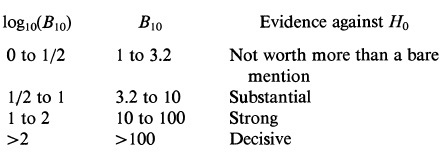
\includegraphics[scale=0.6]{img/BFratios.jpg}
    \caption{Model comparison decision base on BF}
    \label{fig:compRatio}
\end{figure}

\subsection{Application of the Bayesian scheme to our clustering problem}

\subsubsection{Likelihood function and priors}

In this section we simply describe and define the expression of the likelihood function for our application. We also give information on the choice of priors and their respective hyper-parameters.
These expressions will be further detailed when we will express the marginal likelihood.
We will start by discussing the assumed probability distributions of the data in hand.
Our data is described as following:
\begin{itemize}
    \item $Dt$ the global notation for our data set, hence representing all data.
    \item $d=\{1\dots D\}$ represents the dimension of numerical conditions (gene expression profiles).
    \item $l=\{1\dots L\}$ represents the dimension of categorical conditions (clinical variables).
    \item $n=\{1\dots N\}$ the number of samples (patients).
    \item $k=\{1\dots K\}$ the number of clusters.
    \item $X$ represent all numerical variables.
    \item $\Sigma\ =\ {\sigma_1^2\cdots\sigma_D^2}$ the vector representing the noise of each numerical variable.
    \item $\Psi=\{\mu_1\cdots \mu_D\}$ is a vector of gene average values.
    \item $Y$ represent all categorical variables.
    \item $\Phi=\{P(Y_{1}^S)\dots P(Y_{L}^S)\}$ vector of probabilities associated with each possible value for each categorical variable.
\end{itemize}

\emph{Numerical data:}\\
The gene expression profiles are numerical continuous variables, with appropriate normalisation, the probability distribution can be assumed to be normal.
\begin{figure}[!]
    \centering
    \begin{subfigure}[t]{0.25\textwidth}
        \centering
        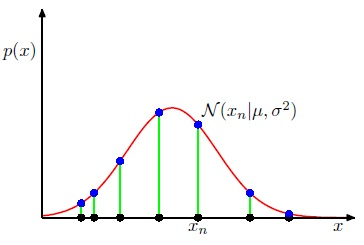
\includegraphics[height=1.2in]{img/gaussDist.jpg}
        \caption{Gaussian distribution, from [bishop]}
    \end{subfigure}%
    \begin{subfigure}[t]{0.25\textwidth}
        \centering
        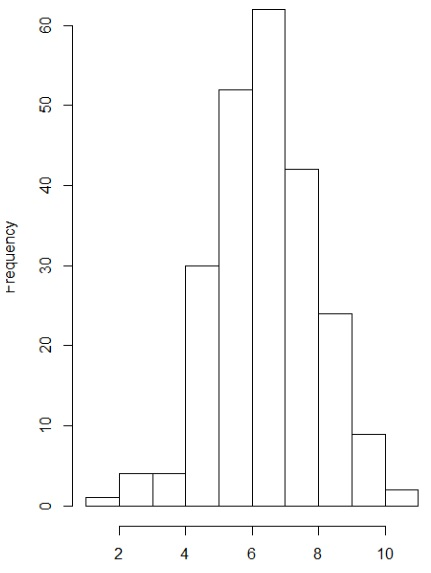
\includegraphics[height=1.2in]{img/distVar.jpg}
        \caption{Histogram of a gene expression profile}
    \end{subfigure}
    \caption{Gaussian distribution assumption}
\end{figure}
Thanks to that assumption we can write the total likelihood function as in equation~\ref{equ:NormalLikelihood}.
Now, if we account for the high dimensional space (several genes), with the joint probability rule it becomes:
\begin{equation}
    \mathcal{L}\ =\ P(X|\Psi,\Sigma)\ =\ \prod_{n=1}^{N}\prod_{d=1}^{D}\mathcal{N}(X_{nd}|\mu_d,\sigma_d^2)
\end{equation}
Choosing a conjugate prior, leads to  an analytical expression for the marginal likelihood.
Here, we only consider a prior on the mean parameter:\\
$$P(\Psi|m,\sigma_0^2)\sim\mathcal{N}(\mu_d|m,\sigma_0^2)$$


In our case, the hyper-parameters are $m=0$ and $\sigma_0^2$ set as the maximum of $\Sigma$.\\

\emph{Categorical variables:}\\
$Y$ follow multinomial distributions, if we take the case of a binomial distribution, particular case of the multinomial distribution, $Y_l\sim\operatorname{B} \left({N, p}\right)$ taking the values $A\ \text{or}\ B$, then the probability of observing the value A is given by:\\
$$P(Y_l=A) = {N\choose k}p^k(1-p)^{N-k}$$


In our case, we can disregard the possible combinations ${N\choose k}$ thank to the independence of the samples, hence the likelihood can be written:
\begin{equation}
    \mathcal{L}=P(Y|\Phi)=\prod_{n=1}^{N}\prod_{l=1}^{L}\prod_SP_{S}^{\delta(Y_{nl},S)}
\end{equation}
Where:
\begin{itemize}
    \item S represents the set of possible value (states) for a given $Y_l$
    \item $\delta$ is the Dirac delta function defined as followed:\\
    \[ \systeme*{1\ \text{if}\ Y_{nl} = S,0\ \text{else}} \]
\end{itemize}
Lets give an easy example, for a dichotomous categorical variable $Y_l$ taking 2 possible values A and B.
Let $P(Y_{l}^A)\ \text{and}\ (1-P(Y_{l}^A))$ be the probability of the event A and B respectively.
$N_A, N_B$ are respectively the number of instances for each value of the variable $Y_1$ Then the likelihood as described in equation (2) will give:\\

$$\mathcal{L}  =  \prod_{1}^{N_A+N_B}\prod_{A,B}P(Y_{l}^A)\cdotp (1-P(Y_{l}^A))$$


Which gives:
\begin{equation}
    \mathcal{L}  =  P(Y_{l}^A)^{N_A}\cdotp (1-P(Y_{l}^A))^{N_B}
    \label{equ:exCat}
\end{equation}
Concerning the prior for the categorical variables, a conjugate prior would be a prior following a Dirichlet distribution, but in our case we simply use a uniform prior equating 1.\\

\emph{Overall likelihood function:}\\
When we regroup the two previous likelihood function under a single expression, and take in consideration the existence of clusters, we obtain the following:
\begin{equation}
    \mathcal{L} = \prod_{k=1}^K\prod_{n\in N_k}\prod_{d=1}^{D}P(X_{knd}|\mu_{kd})\cdotp \prod_{l=1}^{L}\prod_SP_{S}^{\delta(Y_{knl},S)}
    \label{equ:LwithClus}
\end{equation}
Where $N_k$ is the set of index of sample belonging to the cluster $k$.\\
We now move to the heart of the method, the step of marginalisation in order to acquire the likelihood of a given model, leading to the Bayes factor determination.

\subsubsection{Likelihood marginalisation and Bayes factor}

Our method suppose the equiprobability of each clustering model we wish to compare, hence the priors in equation~\ref{equ:BayesRatio} are simplified and the posterior odds directly equate the marginal likelihood ratio between the two models.
We still have to express the marginal likelihood, because we used a Gaussian conjugate prior for the numerical variables, we can use the analytic expression in \cite{murphy}:
\begin{align}
    \mathcal{L}_{Marg} &= P(Dt|m,\sigma^2,\sigma_0^2) \nonumber \\ 
                     &= \int[\prod_{n=1}^N\mathcal{N}(x_n|\mu,\sigma^2)]\mathcal{N}(\mu|m,\sigma_0^2)d\mu
    \label{equ:postuMarph}
\end{align}
So, in the mixed type case, we add the categorical data with $\phi$ the parameter on it:
\begin{equation}
    \mathcal{L}_{Marg}\ =\ \int\prod_{n=1}^N[\mathcal{N}(x_n|\mu,\sigma^2)]\mathcal{N}(\mu|m,\sigma_0^2)\prod_SP_{S}^{\delta(Y_{n},S)}]d\mu d\phi
    \label{equ:Lmarg}
\end{equation}
Because the numerical and categorical variables don't have any parameter in common we can write equation~\ref{equ:Lmarg} as:
\begin{align}
    \mathcal{L}_{Marg}\ =\ \int\prod_{n=1}^N[\mathcal{N}(x_n|\mu,\sigma^2)]\mathcal{N}(\mu|m,\sigma_0^2)]d\mu\cdots \nonumber \\
                    \cdots\int\prod_{n=1}^N[\prod_SP_{S}^{\delta(Y_{n},S)}]P(\phi)d\phi
    \label{equ:Lmarg}
\end{align}
Thus, dissociating the two integral, according a separated treatment for each part.
We will give now the becoming of each integration separately, and reassemble them to obtain the final expression.\\

\emph{Marginal likelihood for numerical variables:}\\
Because we have a high dimension case, then the likelihood correspond to the constant application of the joint probability rule over all conditions.
The marginal likelihood on numerical variables becomes:
\begin{equation}
    \mathcal{L}_{Marg}^{num}\ =\ \prod_{d=1}^D\int\prod_{n=1}^N[\mathcal{N}(x_{nd}|\mu_d,\sigma_d^2)]\mathcal{N}(\mu_d|m,\sigma_0^2)]d\mu_d
\end{equation}
And by expending the expression for all the parameter values we have:
\begin{align}
    \mathcal{L}_{Marg}^{num} &= \int\prod_{n=1}^N[\mathcal{N}(x_n{1}|\mu_1,\sigma_1^2)]\mathcal{N}(\mu_1|m,\sigma_0^2)]d\mu_1\cdots \nonumber \\
    &\int\prod_{n=1}^N[\mathcal{N}(x_{nD}|\mu_D,\sigma_D^2)]\mathcal{N}(\mu_D|m,\sigma_0^2)]\mu_D
\end{align}
It has been shown in \cite{murphy} that the expression in equation~\ref{equ:postuMarph} can be analytically written:
\begin{align}
\mathcal{L}_{Marg} = \frac{\sigma}{(\sqrt{2\pi}\sigma)^N(\sqrt{N\sigma_0^2+\sigma^2})}\exp(\frac{-\sum_{n=1}^Nx_n^2}{2\sigma^2}\nonumber\\
    -\frac{m^2}{2\sigma_0^2})\exp(\frac{\frac{\sigma_0^2N^2\overline{x}^2}{\sigma^2}+\frac{\sigma^2m^2}{\sigma_0^2}+2N\overline{x}m}{2(N\sigma_0^2+\sigma^2)})
\end{align}
In our case we choose $m=0$, and accounting for the multivariate Gaussian distribution it becomes:
\begin{align}
\mathcal{L}_{Marg}^{num} = \frac{1}{(\sqrt{2\pi}^{DN}\prod_{d=1}^D\sigma_d^{N-1}(\sqrt{N\sigma_0^2+\sigma_d^2})}\nonumber\\
    \exp(-\frac{1}{2}\sum_{d=1}^D\sum_{n=1}^N\frac{x_{dn}^2}{\sigma_d^2})\exp(\frac{\sigma_0^2N^2}{2}\sum_{d=1}^D\frac{\overline{x}_d^2}{(N\sigma_0^2+\sigma_d^2)\sigma_d^2})
    \label{equ:multiLmarg}
\end{align}
Finally, applying the \emph{natural logarithm} to equation~\ref{equ:multiLmarg}, it simplifies as:
\small{
\begin{align}\label{equ:lnLikeNum}
ln(\mathcal{L}_{Marg}^{num})= ln(\frac{1}{(\sqrt{2\pi}^{DN}\prod_{d=1}^D\sigma_d^{N-1}(\sqrt{N\sigma_0^2+\sigma_d^2})})\nonumber \\
-\frac{1}{2}\sum_{d=1}^D\sum_{n=1}^N\frac{x_{dn}^2}{\sigma_d^2}+\frac{\sigma_0^2N^2}{2}\sum_{d=1}^D\frac{\overline{x}_d^2}{(N\sigma_0^2+\sigma_d^2)\sigma_d^2}\nonumber\\
= -\frac{DN}{2}ln(2\pi)+\sum_{d=1}^D[\frac{(N-1)}{2}ln(\sigma_d^2)+\frac{1}{2}ln(N\sigma_0^2+\sigma_d^2)]\nonumber\\
-\frac{1}{2}\sum_{d=1}^D\sum_{n=1}^N\frac{x_{dn}^2}{\sigma_d^2}+\frac{\sigma_0^2N^2}{2}\sum_{d=1}^D\frac{\overline{x}_d^2}{(N\sigma_0^2+\sigma_d^2)\sigma_d^2}
\end{align}
}
Using the \emph{natural logarithm} lower the computational time needed and also simplify conveniently the \emph{exponential} in the expression.\\
\emph{Marginal likelihood for categorical variables:}\\
The integral on one categorical variable, seen in equation~\ref{equ:MargMod} can be expended, once again thanks to the joint probability rule, in the multivariate case as:
\begin{align}
    \mathcal{L}_{Marg}^{cat} = \prod_{l=1}^L\int_0^1\prod_{n=1}^N\prod_SP_{S}^{\delta(Y_{nl},S)}P(\phi_l)d\phi_l\nonumber\\
    = \int_0^1\prod_{n=1}^N\prod_SP_{S}^{\delta(Y_{n1},S)}P(\phi_1)d\phi_1\cdots\int_0^1\prod_{n=1}^N\prod_SP_{S}^{\delta(Y_{nL},S)}P(\phi_L)d\phi_L
    \label{equ:LmargCat}
\end{align}
Here we can integrate between 0 and 1 because we are working with probabilities, so if we ignore the prior which always equates 1, we see that the marginal likelihood of each categorical variable is equivalent to a Beta function.
Beta function:\\
$$\textbf{B}(x,y)\ =\ \int_0^1t^{x-1}(1-t)^{y-1}dt$$


We see here that the Beta function fits the expression of the likelihood in the example of equation~\ref{equ:exCat}.
We can easily make the analogy between $t$ and $1-t$ with $P(Y_{l}^A)$ and $(1-P(Y_{l}^A))$.
The difference resides in the parameters of the function, indeed the Beta function deals with $x$ and $y$, which gives $x-1$ and $y-1$ as power of $t$ and $t-1$. In the example it is $N_A$ and $N_B$ which take this role, so we can easily express them together:
\begin{align}
    x &= N_A\ +\ 1\\
    y &= N_B\ +\ 1
\end{align}
So the integral, if expressed with $N_A$ and $N_B$ becomes:\\
$$\textbf{B}(N_A,N_B)\ =\ \int_0^1t^{N_A}(1-t)^{N_B}dt$$


So it perfectly matches with our example. Even in the case of variables with more than two possible events, the Beta function can be generalised in its calculation, using the other definition of the Beta function, closely related to the Gamma function, given by:\\
$$\textbf{B}(x,y)\ =\ \frac{\Gamma(x)\Gamma(y)}{\Gamma(x\ +\ y)}$$


Gamma function:\\
$$\Gamma(n)\ =\ (n-1)!$$


And with our example:\\
$$\textbf{B}(N_A,N_B)\ =\ \frac{\Gamma(N_A+1)\Gamma(N_B+1)}{\Gamma(N_A+N_B+2)}\ =\ \frac{N_A!N_B!}{(N_A+N_B+2)!}$$


When we generalise the expression, we have:
\begin{equation}
    \textbf{B}(Y_l)\ =\ \frac{\prod_{j=1}^J\Gamma(N_{Y_l=j}+1)}{\Gamma(N+sup(S_l))}\ =\ \frac{\prod_{j=1}^JN_{Y_l=j}!}{(N+sup(S_l))!}
\end{equation}
With $S_l$, the set of possible events of the variable $Y_l$, $N$, the number of samples, $j$ iterating over the set $S_l$.
Thus, from equation~\ref{equ:LmargCat}, we can write the likelihood:
\small{
\begin{equation}
     \mathcal{L}_{Marg}^{cat} = \frac{\prod_{j_1=1}^{J_1}\Gamma(N_{Y_1=j_1}+1)}{\Gamma(N+sup(S_1))}\cdots\frac{\prod_{j_L=1}^{J_L}\Gamma(N_{Y_L=j_L}+1)}{\Gamma(N+sup(S_L))}
     \label{equ:LmargCatfin}
\end{equation}
}
Then, for convenience and for saving computational resources, we apply the \emph{natural logarithm} to equation~\ref{equ:LmargCatfin}:
\small
\begin{align}
    \mathcal{L}_{Marg}^{cat}\ =\ \sum_{j_1=1}^{J_1}ln(\Gamma(N_{Y_1=j_1}+1))-ln(\Gamma(N+sup(S_1)))+\cdots\nonumber\\
 \cdots+\sum_{j_L=1}^{J_L}ln(\Gamma(N_{Y_L=j_L}+1))-ln(\Gamma(N+sup(S_L))) 
\end{align}

\emph{Total marginal likelihood:}\\
So if we bind the two parts together:
\begin{equation}
    ln(\mathcal{L}_{Marg})\ =\  ln(\mathcal{L}_{Marg}^{num})\ +\ ln(\mathcal{L}_{Marg}^{cat})
    \label{equ:finalLmargTot}
\end{equation}
Notice that the marginal likelihood expressions are given considering only one cluster, but as shown in equation~\ref{equ:LwithClus}, accounting for more than one cluster would simply require to add a sum over all clusters and change the total number of sample into the number of sample in each respective cluster.\\

\emph{Bayes Factor:}\\
Now that we have the expression of the marginal likelihood over the respective parameters, which, once marginalised gives the likelihood of a given model, we can simply get the BF by applying the ratio (bocoming a difference with $ln$) between two models 1 and 2:
\begin{equation}
    ln(BF_{12})\ =\ ln(\mathcal{L}_{Marg}^{M1})\ -\ ln(\mathcal{L}_{Marg}^{M2})
    \label{equ:lnLikeBF}
\end{equation}
And from the results and the information given in figure~\ref{fig:compRatio}, we can see which one of the two models fits our data the better.
From this value, we can directly compare clustering results from any algorithm, and we can also create a clustering method based on the behaviour of the BF, hence deciding to merge of samples together or not based on the value of the BF.

\subsection{Proposed Methods}

We want here to present different implementations, based on the BF scheme.
Concerning the algorithms, only one was successfully implemented but the reasoning behind the other ones will be explained as well.

\subsubsection{Bayes Factor calculation from clustering result}

The first, and simplest, implementation reside in the simple calculation of the BF from a list of already clustered and labeled data.
The source code can be found in supplementary file.
Here we simply feed the function with two clustering results, one with 3 clusters and the other with 4 for instance, we also give it the data set it is from and it return the BF after calculation of the numerical and categorical marginal likelihood separately.
This implementation is able to deal with missing values, it basically replace them by zeros when calculation, hence missing values don't participate in the marginal likelihood calculations.

The source code of all implementation is given in supplementary files.

\subsubsection{Hierarchical Bottom-Up clustering Algorithm}

The first hierarchical algorithm takes a bottom-up approach, which means it starts by assuming all the samples as distinct clusters and merge them at each step until all the samples are gathered in a single cluster.
In this algorithm, we consider all possible combinations, meaning that the tree will not be reduced as a binary one, more than two branches association is possible.
At each step of the algorithm, the marginal likelihood ($\mathcal{L}_{Marg}$) between each pair of samples is computed, then the samples maximising $\mathcal{L}_{Marg}$ are taken and merged together into one cluster. That decision comes from the fact that maximising the $\mathcal{L}_{Marg}$ means maximising the fitness to the observed data.
The matrix is then updated to reflect the new assumed model, accounting for the freshly created cluster.
The calculation of such matrix requires the marginal likelihood of the previous assumed model, we show that a mathematical simplification on the likelihood expression can be used for the first algorithm's iteration.
Indeed, a lot of calculation is unnecessary for our purpose, which allows us to simplify the expression, hence simplifying the calculation, reducing the required computational resources.
Lets detail the mathematical simplifications, which will be used in the other implemented methods as well.
First of all, we will use the following notation by convenience:
\begin{itemize}
    \item $a=-\frac{DN_k}{2}ln(2\pi)+\sum_{d=1}^D[\frac{(N_k-1)}{2}ln(\sigma_d^2)+\frac{1}{2}ln(N_k\sigma_0^2+\sigma_d^2)]$
    \item $b=-\frac{1}{2}\sum_{d=1}^D\frac{x_{d}^2}{\sigma_d^2}$
    \item $c=\frac{\sigma_0^2N_k^2}{2}\sum_{d=1}^D\frac{\overline{x}_d^2}{(N_k\sigma_0^2+\sigma_d^2)\sigma_d^2}$
    \item lets call $d$ the categorical part of the marginal likelihood
    \item $d\ =\ \sum_{s=1}^S[ln(\Gamma(N_s))]\ -\ ln(\Gamma(N+sup(S)))$
    \item taking even more liberties, we can note $a(N_k=1)$ corresponding to a but with $N_k$, number of samples in the cluster k, equals 1.
    \item In the same way, $b(x_n),\c(x_n)\ \text{and}\ d(x_n)$ respectively the part b, and d taking the value of the sample $x_n$ for their calculation.
\end{itemize}
a,b and c come from equation~\ref{equ:lnLikeNum}, just without the sum over all samples.
The first step is to calculate the marginal likelihood of the model 0, the model assuming each sample as its own cluster. In such scheme, $N_k$ would equates 1, and the sample mean in c directly equates the sample value by gene. Furthermore, d also gives great simplification because the numerators in equation~\ref{equ:LmargCatfin} becomes 0 with \emph{ln}.
Hence we get:
\begin{equation}
    \mathcal{L}_{Marg}^{M0}\ =\ N\cdotp a(N_k=1)\ +\ \sum_{n=1}^Nb(x_n)\ +\ \sum_{n=1}^Nc(x_n)\ +\ \sum_{n=1}^Nd(x_n)
    \label{equ:M0}
\end{equation}
Now if we desire to have the marginal likelihood of any pair of samples i and j:
\begin{align}
    \mathcal{L}_{Marg}^{ij}\ =\ (N_k-2)a(N_k=1)\ +\ a(N_k=2)\ +\ \sum_{n=1}^Nb(x_n)\nonumber\\
    +\ \sum_{N\setminus{i,j}}c(x_n) +\  c(\overline{x_ix_j})\ +\ \sum_{N\setminus{i,j}}d(x_n)\ +\ d(x_i,x_j)
\end{align}
We then can express it using $\mathcal{L}_{Marg}^{M0}$:
\begin{align}
    \mathcal{L}_{Marg}^{ij}\ =\ \mathcal{L}_{Marg}^{M0}\ -\ 2a(N_k=1)\ +\ a(N_k=2)\ +\ \sum_{n=1}^Nb(x_n)\nonumber\\ +\ c(\overline{x_ix_j}) -\ c(x_i)\ -\ c(x_j)\ +\ d(x_i,x_j)\ -\ d(x_i)\ -\ d(x_j)
\end{align}
So for each sample pairs, the difference resides only in the parts depending on $x_i$ and $x_j$, the rest can be considered constants and ignored, which gives finally:
\begin{align}
    \mathcal{L}_{Marg}^{ij}\ \propto\ c(\overline{x_ix_j})\ -\ c(x_i)\ -\ c(x_j)\ +\ d(x_i,x_j)\nonumber\\ -\ d(x_i)\ -\ d(x_j)
    \label{equ:simplifMath}
\end{align}
The simplification is possible only for the first iteration, after the first merging, it falls due to the unpredictability of possible sample associations.
The lack of such generalised simplification makes the algorithm time complexity too high (exponential), the marginal likelihood matrix having to be updated after the creation of each cluster.
Another version of this algorithm was under development, with main difference a binary tree forcing approach in order to keep the simplification applicable at each step.
Unfortunately, as soon as the number of clusters becomes odd, the simplification falls and complications arise.
\RestyleAlgo{boxruled}
\begin{algorithm}[!]
 \SetKwFunction{UpdateMatrix}{updateMatrix}
 \SetKwInOut{Input}{input}\SetKwInOut{Output}{output}
 \Input{$Dt = (N,D+L)$, $\sigma^2$, prior hyper-parameters (HP)}
 \Output{A list of cluster solutions associated with respective BF}
 \BlankLine
 $L_M\ \leftarrow L_{Marg}^{M0}$\\
 $Cl \leftarrow$ list of clusters (each sample at first)\\
 $N_k$ $\leftarrow$ vector of number of samples by cluster (only 1s at first)\\
 \tcp{Create the first marginal likelihood matrix}
 $L_{Mat}\ \leftarrow$ call \UpdateMatrix{$Cl,\ N_k,\ Dt,\ \sigma^2$, HP}\\
 $K\ \leftarrow$ N\\
 \BlankLine
 \While{we have more than one cluster}
    {
        Get the samples names of the maximum in $L_{Mat}$\\
        Update Cl by merging the two samples\\
        Update $N_k$ as well\\
        Compute the marginal likelihood of the new model\\
        Calculate the Bayes Factor\\
        Replace $L_M$ by the new model $L_M$\\
        \UpdateMatrix{$Cl,\ N_k,\ Dt,\ \sigma^2$, hyper-parameters}\\
        K = K - 1
        Result $\leftarrow$ Append(Cl,K,BF)\\
    }
    Return Result
 \caption{BF\_HC\_Asc}
\end{algorithm}
\RestyleAlgo{boxruled}
\begin{algorithm}[!]
\SetKwInOut{Input}{input}\SetKwInOut{Output}{output}
 \Input{Cl,$N_k$,$Dt = (N,D)$, $\sigma^2$,HP}
 \KwData{List of clusters, each sample value vector}
 \KwResult{Marginal likelihood matrix}
 \tcp{Create a matrix filled with NAs}
 $L_{Mat}\ \leftarrow matrix(NA)$\\
 \For{i in 1 to the number of clusters-1}
    {
        \For{j in i+1 to the number of cluster}
        {
            $L_{Marg}^{ij}\ \leftarrow$ Compute the the marginal likelihood between clusters i and j\\
            \tcp{Put the value into the corresponding index of the new matrix}
            $L_{Mat}[i,j]\ \leftarrow\ L_{Marg}^{ij}$
        }
    }
    Return $L_{Mat}$
 \caption{UpdateMatrix}
\end{algorithm}
The function updating the matrix return a $N\text{x}N$ matrix with the lower triangle filled with $NAs$.
This algorithm is able to deal with missing values.

\subsubsection{Hierarchical Top-Down clustering Algorithm}

The second implementation is a hierarchical Top-down algorithm, which means, we start with all samples gathered in a single cluster and at each step we divide it in smaller clusters based on some conditions.
The work-flow of this algorithm is pretty straightforward and uses the Gower distance, from the "Cluster" package under R, in addition to marginal likelihood.
This approach allow us to avoid having to re-calculate a huge matrix, hence saving a lot of computation time, but it also presents an imperfection, the choice of the dividing condition.
Indeed, each time we want to split a given cluster in two different ones, we face some troubles like, what will be the rule of division or which cluster to divide first.
Unfortunately it is of great difficulty to predict the behaviour of the marginal likelihood, hence finding a relevant way of splitting a cluster is challenging.
For lack of anything better, the splitting condition was set to simply divide a cluster into two equally, or almost equally (case of odd number of samples), sized clusters. 
This separation relies on two steps:
\begin{enumerate}
    \item Calculate the Gower distance matrix for each cluster and get one of the two samples having the maximum distance, we call that sample the \emph{reference sample}
    \item Compute the marginal likelihood between the \emph{reference sample} and all the remaining samples
\end{enumerate}
Through that method, we get, for each singular cluster, the maximum Gower distance and one of the sample associated with it.
We can then sort by decreasing order these distances, which will give us the order of cluster splitting.
This assumption is simple but logical, indeed, the cluster containing the two most distant samples is the strongest candidate for being split in first.
Once we have that list, we just have to iterate on it and calculate for each respective cluster the marginal likelihood combinations.
We then, once again use a decreasing order sorting to basically obtain on the first position the closest samples and at the latest positions the farthest ones.
Finally, we split in two, taking the $floor(\frac{N_k}{2})$ first samples (so if odd number, take the inferior integer), and associate them with the \emph{reference sample} to create a new cluster, the remaining samples are associated into a second new cluster.
At each new iteration over the ordered list, we compute the marginal likelihood of the changed model (one more cluster to take into consideration), and compute the BF with the former model.
Here the first assumed model is as following (all sample in one cluster):
\begin{align}
    \mathcal{L}_{Marg}^{M0}\ =\ a(N_k=N)\ +\ \sum_{n=1}^Nb(x_n)\nonumber\\ 
    +\ c(\overline{x_1\cdots x_N})\+d(x_1,\cdots,x_N)
\end{align}
And when calculating the marginal likelihood with a \emph{reference sample}, the mathematical simplification can go even further than in equation~\ref{equ:simplifMath}, indeed here $x_i$ will be the same for all, $x_{ref}$, so we can consider it a constant and ignore it, which leads to:
\begin{equation}
    \mathcal{L}_{Marg}^{ref,j}\ \propto\ c(\overline{x_{ref}x_j})\ -\ c(x_j)\ +\ d(x_{ref},x_j)\ -\ d(x_j)
\end{equation}
\RestyleAlgo{boxruled}
\begin{algorithm}[!]
 \SetKwInOut{Input}{input}\SetKwInOut{Output}{output}
 \Input{$Dt = (N,D+L)$, $\sigma^2$, prior hyper-parameters (HP), number of  maximum desired clusters}
 \Output{A list of cluster solutions associated with respective BF}
 \BlankLine
 $old.L_M\ \leftarrow L_{Marg}^{M0}$\\
 $Cl \leftarrow$ list of clusters (a single cluster with all samples)\\
 \tcp{K accounts for the number of clusters, 1 at first}
 $K\ \leftarrow$ 1\\
 \BlankLine
 \While{We haven't reached the desired number of clusters}
    {
        gower $\leftarrow$ Compute the Gower distance matrix of each cluster\\
        gower.max $\leftarrow$ fetch the reference sample and the distance value for each cluster\\
        \tcp{sort the values by decreasing order}
        gower.max.ord $\leftarrow$ sort(gower.max)\\
        indices $\leftarrow$ clusters indices in the order given by gower.max.ord\\
        \For{i in indices}
        {
            Take the cluster to split in Cl\\
            Compute the marginal likelihood with the reference sample\\
            cl.split $\leftarrow$ newly formed clusters\\
            cl.remaining $\leftarrow$ clusters not split yet\\
            K $\leftarrow$ K+1\\
            \tcp{Marginal likelihood of model k}
            $new.L_M\ \leftarrow$ compute model marginal likelihood\\
            \tcp{$old.L_M$ equates $L_{Marg}^{M_{K-1}}$}
            BF $\leftarrow$ $old.L_M\ -\ new.L_M$\\
            Update Cl\\
            Result $\leftarrow$ append Cl and BF
        }
    }
    Return Result
 \caption{BF\_HC\_Desc}
\end{algorithm}
This algorithm is also able to deal with missing values in the same manner as the first one.

\subsubsection{Simplified hierarchical Bottom-Up clustering Algorithm}

The last implemented algorithm is also a bottom-up one, but in order to minimise the overall time complexity, only the first marginal likelihood matrix is calculated and all clusters are formed from it.
This algorithm is of really simple design, the idea is to feed it with a desired number of cluster and it will stop once this number is reached.
At first, the algorithm calculate the marginal likelihood matrix as in the first step of the first algorithm, using the mathematical simplification shown earlier.
Then, from this matrix it will fetch at each step the maximum and the two samples corresponding to put them together in a single cluster. Once it is done, it puts NA into the index of this maximum, which allows to avoid taking the same samples twice.
Because of the possibility of getting samples already in a cluster formed at a previous step, it is necessary to add a checking task, which behaves differently according to the case we are in:
\begin{itemize}
    \item if the two samples are already in the general cluster solution
        \begin{enumerate}
            \item Get the respective cluster index already comprising these samples.
            \item Merge these two clusters into one.
        \end{enumerate}
    \item if only one of the sample is already in a cluster
        \begin{enumerate}
            \item Identify which of the two is already in a cluster.
            \item Get the index of the corresponding cluster
            \item Add the second sample into that cluster
        \end{enumerate}
    \item if none of the samples are already in an existing cluster, we simply put them together in a new cluster
\end{itemize}
By following this work-flow, and looping it until all samples are put into a unique cluster, we obtain the final cluster solution.
Unfortunately, a flaw in the design made it difficult to get the desired result, being able to both cluster all samples and to put them into a given number of clusters was not as easy as anticipated.
By lack of time some issues were not fully addressed, leading to poor results, the algorithm having tendencies to stop before clustering all samples and creating really unbalanced clusters with generally a big one regrouping most of the samples and the remaining ones having a handful number of samples.
\RestyleAlgo{boxruled}
\begin{algorithm}[!]
 \SetKwFunction{UpdateMatrix}{updateMatrix}
 \SetKwFunction{MergeBoth}{mergeBoth}
 \SetKwFunction{MergeOne}{mergeOne}
 \SetKwInOut{Input}{input}\SetKwInOut{Output}{output}
 \Input{$Dt = (N,D+L)$, $\sigma^2$, prior hyper-parameters (HP), number of clusters desired}
 \Output{A cluster solution associated with its BF}
 \BlankLine
 $L_M\ \leftarrow L_{Marg}^{M0}$\\
 $Cl \leftarrow$ list of clusters (each sample as cluster)\\
 $N_k$ $\leftarrow$ vector of number of samples by cluster (only 1s)\\
 $L_{mat}\ \leftarrow$ \UpdateMatrix{Cl,$N_k$,Dt,$\sigma^2$,HP}\\
 \tcp{List containing the general cluster solution, will be update at each iteration}
 $Cl.sol\ \leftarrow$ void list\\
 \BlankLine
 \While{We haven't reached the desired number of clusters}
    {
       samp.max $\leftarrow$ samples associated with max($L_{mat}$)\\
       \tcp{if we note i and j indices of the current maximum}
       $L_{mat}[i,j]\ \leftarrow$ NA\\
       \If{both samples already in Cl.sol}
       {
        Cl.sol $\leftarrow$ \MergeBoth{Cl.sol,samples}\\
       }
       \uElseIf{Only one sample already in Cl.sol}
       {
        CL.sol $\leftarrow$ \MergeOne{Cl.sol,samples}\\
       }
       \Else
       {
        \tcp{None of the samples are already in Cl.sol}
        Cl.sol $\leftarrow$ Append in a new index the two samples\\
       }
    }
    $L_{marg}\ \leftarrow$ Compute marginal likelihood of the model\\
    BF $\leftarrow\ L_M\ -\ L_{marg}$\\
    Cl.sol $\leftarrow$ Append Cl.sol with BF\\
    Return CL.sol
 \caption{BF\_HC\_Asc\_s}
\end{algorithm}
\RestyleAlgo{boxruled}
\begin{algorithm}[!]
 \SetKwInOut{Input}{input}\SetKwInOut{Output}{output}
 \Input{Cluster list, two samples to add}
 \Output{A new list containing all clusters}
 \BlankLine
 \For{loop on each element of the clusters list}
 {
  \If{one of the samples is in the current cluster}
  {
   indices $\leftarrow$ Get the index of this cluster\\
  }
  \Else
  {
   Do nothing\\
  }
 }
 Merge the two clusters corresponding to indices into one\\
 return the new cluster solution
 \caption{MergeBoth}
 \label{algo:merge}
\end{algorithm}
The function \emph{MergeOne()} acts like in algorithm~\ref{algo:merge}, but directly puts the sample not already clustered in the cluster containing the other sample.
These functions avoid getting duplicated samples and clusters.

\section{Results}

\subsection{Method testing}

In order to assess the performance of the methods, we applied them to different data sets found on \cite{source1} and \cite{source2}.
We used them to investigate the computational time required by our methods, and because we know the true classes for some of the data sets, we were also able to appreciate their accuracy.
The list and description for each data set can be seen in table~\ref{tab:testDT}:
\begin{table}[!]
    \centering
    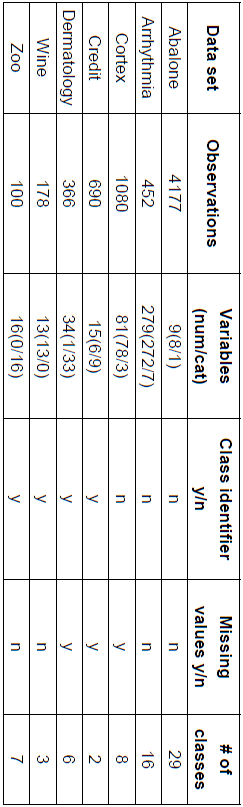
\includegraphics[scale=0.4]{img/dataSets.png}
    \caption{Data sets used for testing our methods}
    \label{tab:testDT}
\end{table}
We chose these data sets in order to consider different possibilities, hence we have data sets with both categorical and numerical variables, but also the Wine data set with only numerical, opposed to the Zoo one having only categorical variables.
They also offer different dimensions, which allow us to explore the time required by the algorithms to perform.

\subsubsection{Bayes Factor induced clustering}

For comparison purpose, we decided to apply another already existing method to the same data sets. As stated before, the Gower distance can be used on mixed type of data, then applying a simple hierarchical clustering algorithm, available under R with the \emph{hclust()} function, with either Ward or Complete method of linkage (equations~\ref{equ:comp},\ref{equ:ward}).
We applied the same linkage method but instead of the Gower distance matrix, we calculated the Marginal likelihood matrix between each possible sample pairs.
We are interested in finding the right number of classes, the accuracy, and the computational time required.
\begin{table}[!]
    \centering
    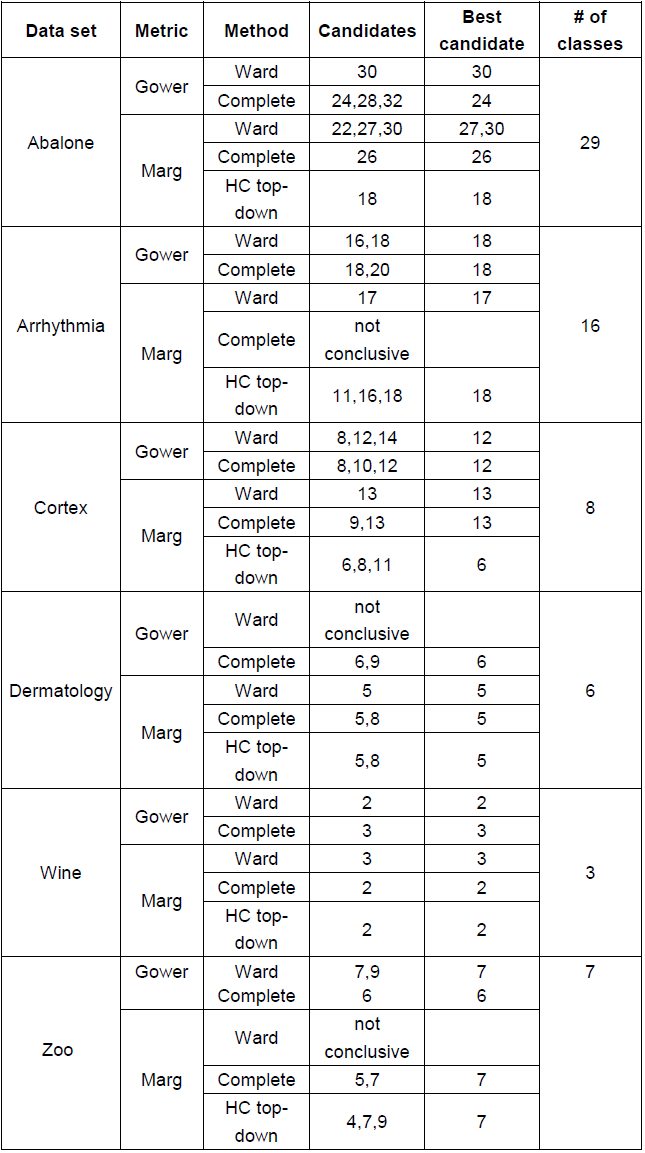
\includegraphics[scale=0.35]{img/ResultsTable.png}
    \caption{Table of results for Gower and Marginal likelihood metrics}
    \label{tab:ResTab}
\end{table}
In table~\ref{tab:ResTab}, \emph{Candidates} represent the cluster models which represent good candidates for the best cluster model and \emph{\# of classes} is the true number of classes in the data set.
The results obtain in table~\ref{tab:ResTab}, were found by plotting the BFs for each model, determining candidates model, and in the case were several candidates were found, comparing the BFs between candidates to find the best one.
Only the algorithm top-down was used, because the bottom-up ones lacked optimisation or yielded really poor clusters.
As this table shows, all techniques manage to get pretty close or even equalise the true number of classes in the data sets, so we consider that the ability of our implemented methods to discover the right number of clusters is satisfying.
\begin{figure}[!]
    \centering
    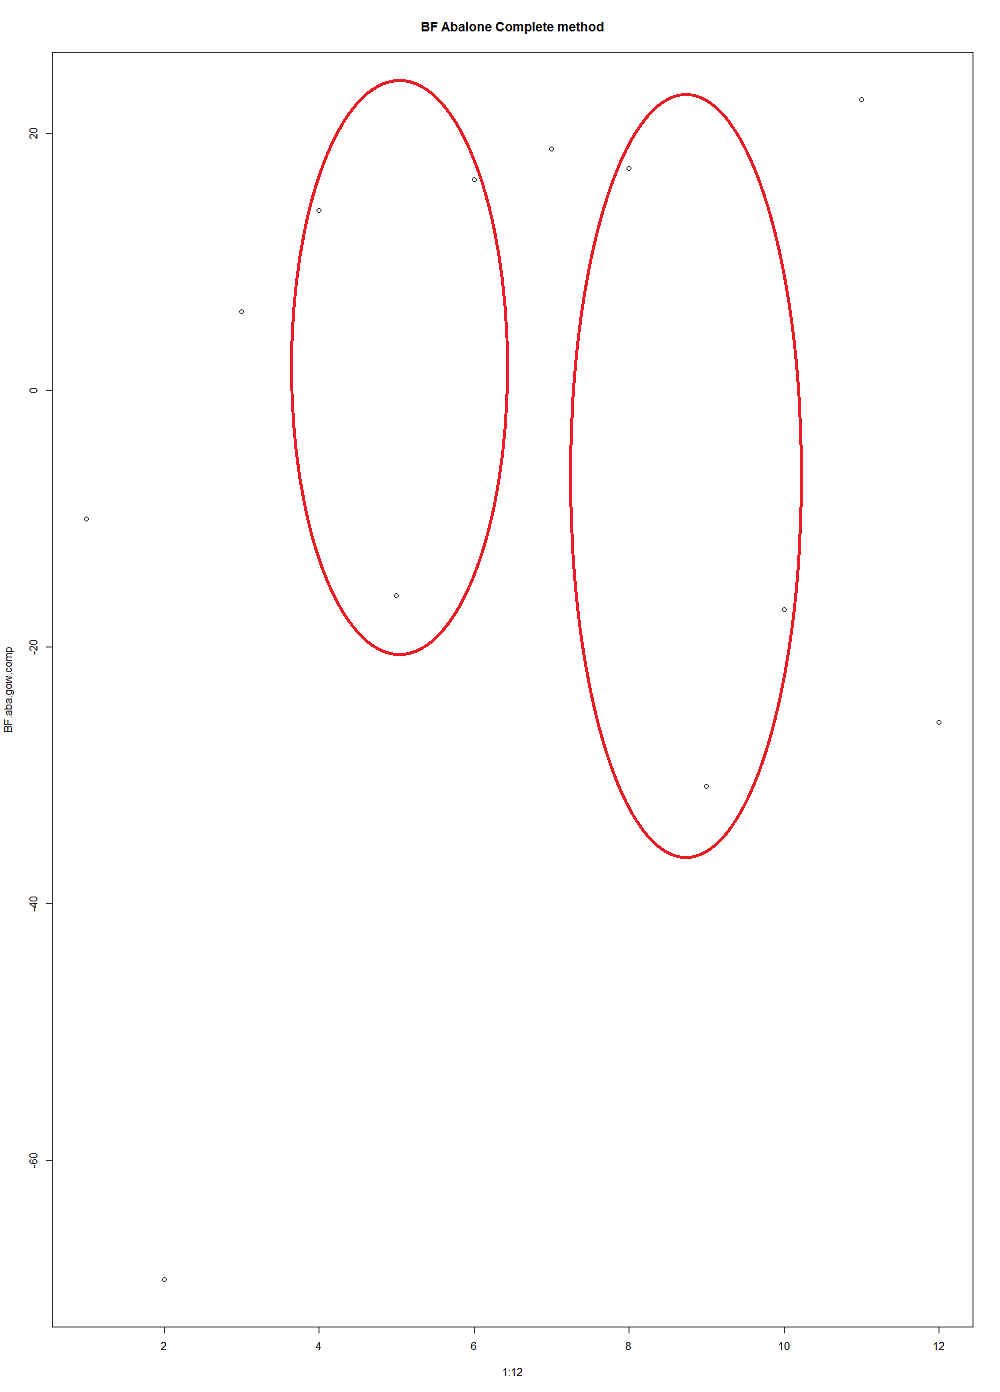
\includegraphics[scale=0.3]{img/BFplot.png}
    \caption{Conclusive example of BF plot interpretation}
    \label{fig:BFplotConclusive}
\end{figure}
Figure~\ref{fig:BFplotConclusive} shows how we choose the candidate models. From equation~\ref{equ:lnLikeBF} and because each dot represent the log BF between the previous and the current model, i.e: 2 clusters vs 3 clusters, we concluded that when the dot is below zero, it means that the current model is better than the previous one. Furthermore, when after going below zero the next dot goes in higher values (the current model becomes the former one for this dot), it confirm that the "new" former model is better.
We also noticed that even when not going below zero, but showing the same pattern can also predict a good candidate, as shown in figure~\ref{fig:notbelowzero}, there are two candidates not giving a log BF below zero, but are actually better than the one going below zero.
\begin{figure}[!]
    \centering
    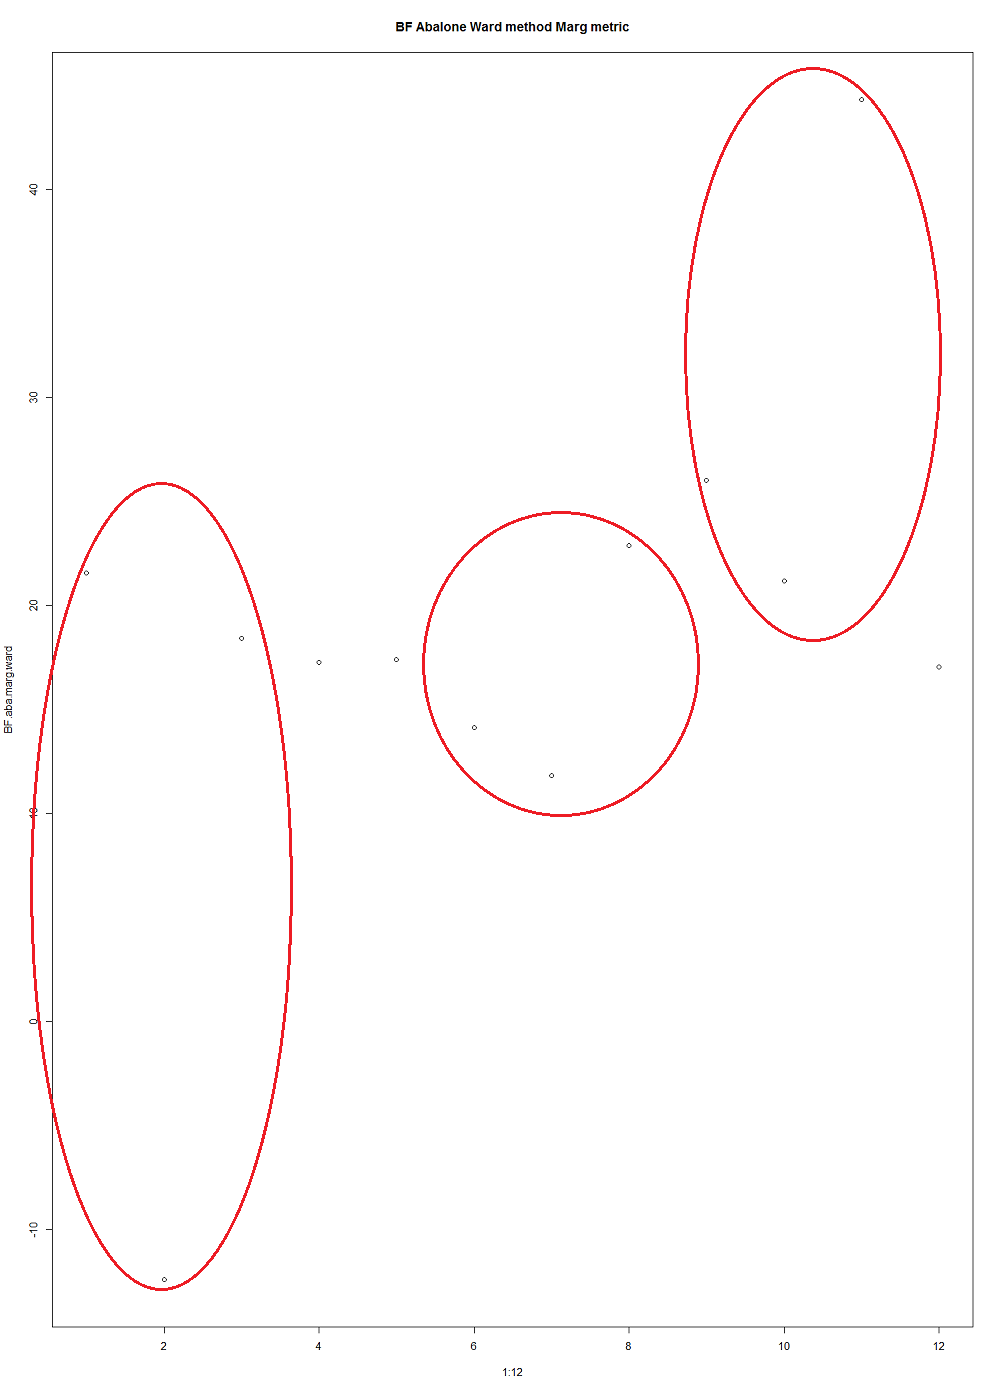
\includegraphics[scale=0.3]{img/BFplotNotBelowZero.png}
    \caption{Conclusive example with less obvious candidates}
    \label{fig:notbelowzero}
\end{figure}
Most of the BF were strong or decisive according to figure~\ref{fig:compRatio}. Only for the data set Abalone we got a substantial result between the 22 cluster model and the 27 one, and a not worth even a bare mention case between 27 clusters and 30 clusters, which is why we considered them both as best candidates.

\subsubsection{Accuracy results}

Some data sets have well defined class identifiers, allowing us to compute the accuracy of the different methods.
In order to determine the accuracy, we simply used the Jaccard's index between the true classes and the clustering results. 
For two sets A and B, the Jaccard's index can be calculated with:
\begin{align}
    Jaccard(A,B)\ =\ \frac{|A\cap B|}{|A\cup B|}
\end{align}
So, this index is merely a similarity measure between two sets.
In table~\ref{tab:accTable}, we put a summary of the results, putting only the maximum Jaccard index found for the respective method used and for each class.
Our results show that the accuracy using the Gower distance matrix and the log marginal likelihood matrix share the lead, depending on the data set considered.
However, our hierarchical top-down clustering method perform poorly and rarely goes over an index value of 0.5.
\begin{table}[!]
    \centering
    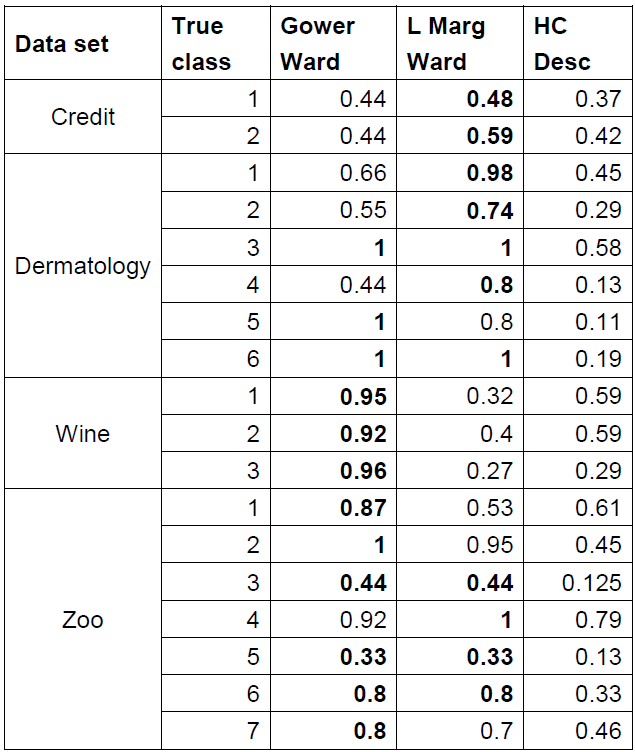
\includegraphics[scale=0.4]{img/AccTable.png}
    \caption{Table of maximum Jaccard index by method}
    \label{tab:accTable}
\end{table}
Although our methods are able to find the right number of clusters, we showed here that the accuracy is not really on point, especially for the hierarchical top-down algorithm we implemented.

\subsection{Results on the lung adenocarcinoma data sets}

Even thought the test were not conclusive, and accurate enough, we applied our methods to different data sets to see if we could still find interesting results.
We used the 4 data sets described earlier in section~\ref{sec:preprocess}, and obtain the results shown in table~\ref{tab:resAdeno}.
We can see that in most cases, our methods find a best cluster solution of two clusters, but as it has been previously determined in \cite{hayes}, \cite{wilk} and \cite{TCGA}, the number of sub-types is at least three. From there, we can assume that, unfortunately, our scheme is not sensitive enough, and pushing the investigation further would not really lead to meaningful outcomes.
In the case of the TCGA data sets, because we have access to the classification made in \cite{TCGA}, we just can have a look at the accuracy yielded by the different gene sets taken into consideration, which would, at least, give us which gene set would seem to be a better predictor to lung Adecarcinoma sub-types exploration.
\begin{table}[!]
    \centering
    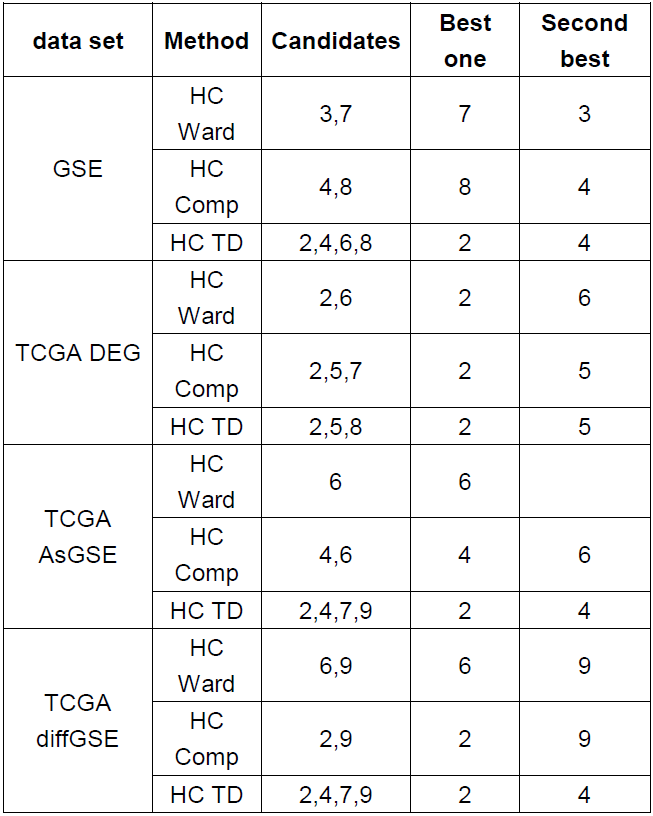
\includegraphics[scale=0.4]{img/ResultsAdeno.png}
    \caption{Clustering results with the lung Adenocarcinoma data sets}
    \label{tab:resAdeno}
\end{table}
\begin{table}[!]
    \centering
    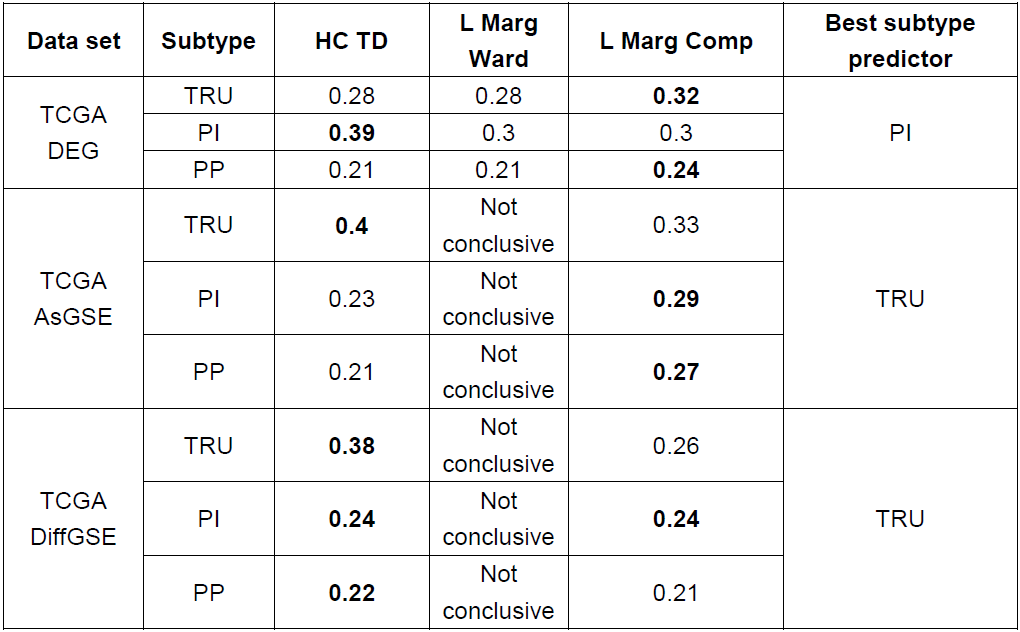
\includegraphics[scale=0.3]{img/AccAdeno.png}
    \caption{Methods Accuracy on Adenocarcinoma TCGA data sets}
    \label{tab:accadeno}
\end{table}
Our analysis about accuracy, shown in table~\ref{tab:accadeno}, was produced by taking a three clusters solution from our different methods.
Although it yielded poor results, especially the Ward method being often inconclusive due to an aggregation of most of the samples into one cluster, we still can see that the differentially expressed gene set is a decent predictor for the PI sub-type, where the gene set in "AsGSE" is a decent predictor for the TRU sub-type. Unfortunately, none of the considered gene sets were able to be good enough predictor for the PP sub-type.
Further analyses have not been conducted, deemed to be unnecessary given such inconclusive results.
This is why, we consider our methods as a framework, laying the foundations for future research using the same scheme but bringing some tuning to our model.

\subsection{Time Complexity}\label{sec:tps}

Optimisation is a very important feature in computer science, being able to implement an algorithm computing quickly is a great challenge.
We have shown how we could simplify the mathematical model to avoid some unnecessary calculation, and because we used R, we can also talk about some optimisation problem we had.
R software is far from being an optimal environment for algorithmic implementations, especially under Windows. Even if some tools like R open for Windows or the package "Parallel", for Mac OS or Linux distributions, allow parallel computing, not all functions in R profit from it.
Furthermore, the handling of objects is not really practical, often reduced to use lists for simplification purpose.
So, overall, coding an algorithm with R asks additional reflections and adaptations in order to minimise the computational time consumption.
In table~\ref{tab:runTime}, the time required for each case is given, and as we can see, the Marginal likelihood matrix is a quite time consuming process.
For huge data sets, we quickly reach several hours of computational time, which is not desirable.
These results were obtained with an Intel Core i7-3970X 3.50GHz processor, 32GB of RAM under Windows 7 Ultimate 64-bits.
At first glance, we see that the number of samples play a more important role in the time consumption than variables.
Indeed, if we look at the time required for the GSE data set (442 observations, 2249 variables) and for the TCGA DEG one (230, 2858), we notice a huge difference even though the TCGA data set has 600+ variables more than GSE for only 200+ less observations.
We confirmed that idea by varying the number of observations with a constant number of variables and doing the opposite for the marginal likelihood matrix calculation, which is shown in figure~\ref{fig:tpsObs} and \ref{fig:tpsVar}.
Indeed, from these figures, wee observe that the time consumption increase linearly when varying the variable number only, and takes the form of a quadratic equation when varying the observations only.
So, the overall time consumption when varying the number of observations and variables together give the figure~\ref{fig:tpsBoth}.
The time complexity given in function of N (number of samples) for our implementations is:
\begin{itemize}
    \item Marginal likelihood matrix: $O(N^2)$
    \item Top-Down clustering algorithm: $O(N)$
\end{itemize}
\begin{table}[!]
    \centering
    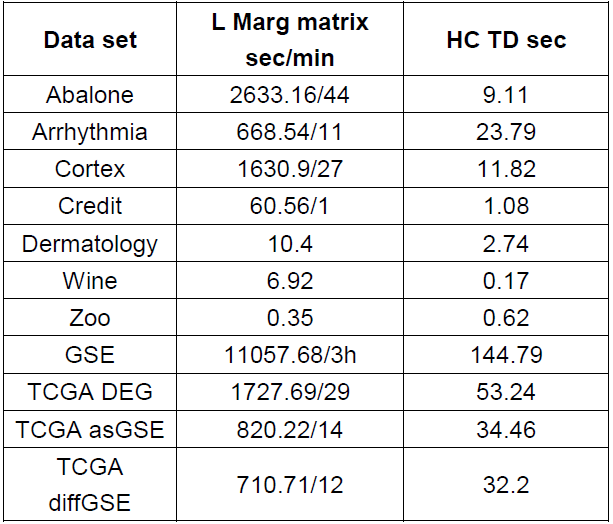
\includegraphics[scale=0.4]{img/runTime.png}
    \caption{Computational time by data set for each method}
    \label{tab:runTime}
\end{table}
\begin{figure}[!]
    \centering
    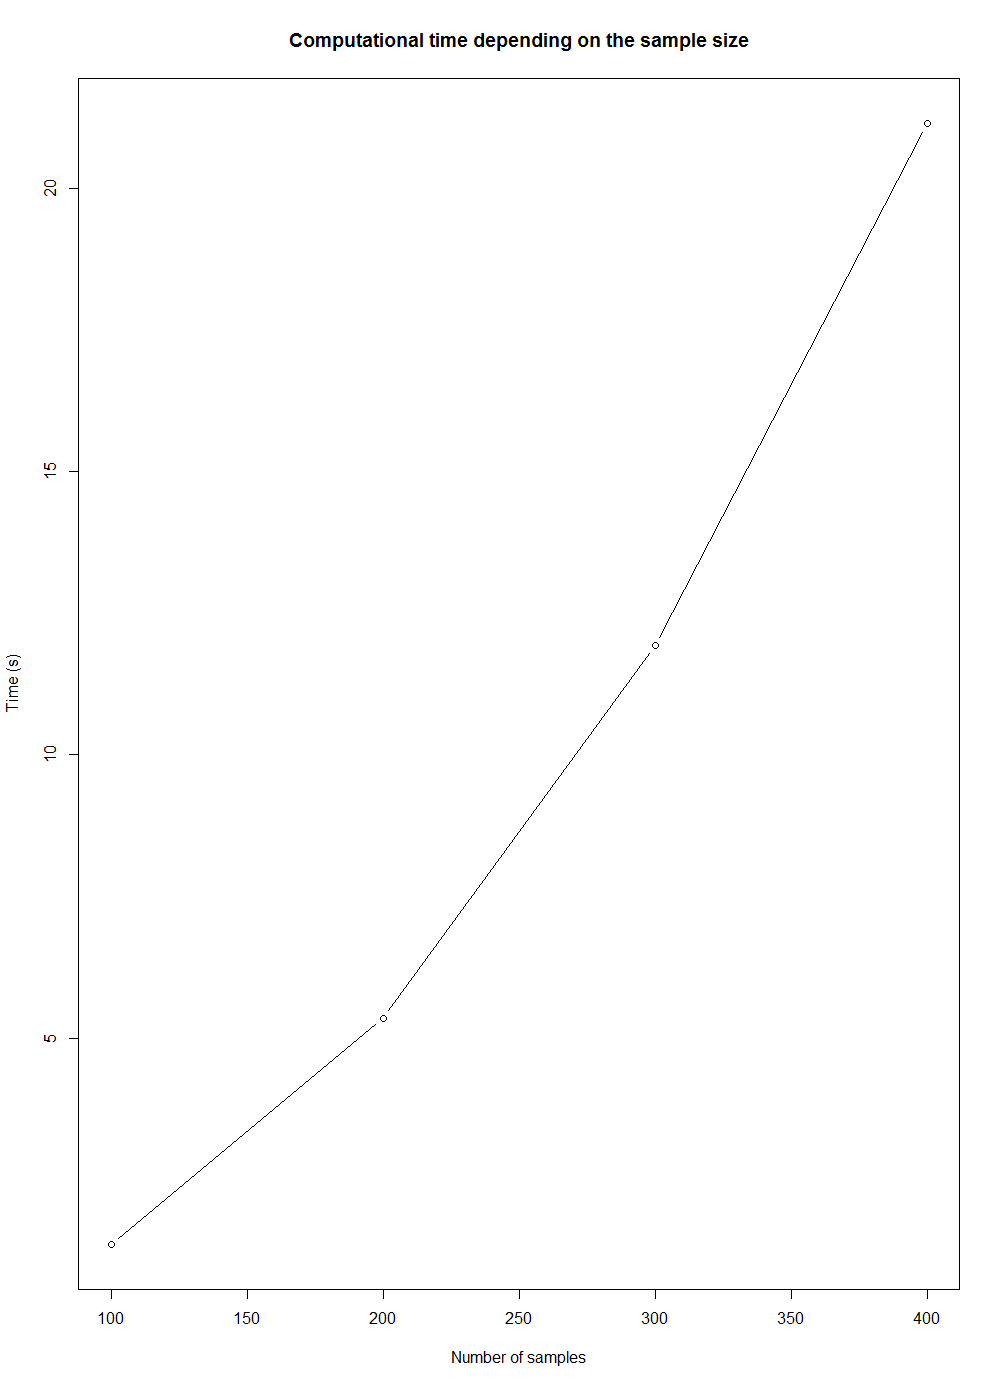
\includegraphics[scale=0.3]{img/ObsTime.png}
    \caption{Time consumption evolution in function of number of observations}
    \label{fig:tpsObs}
\end{figure}
\begin{figure}[!]
    \centering
    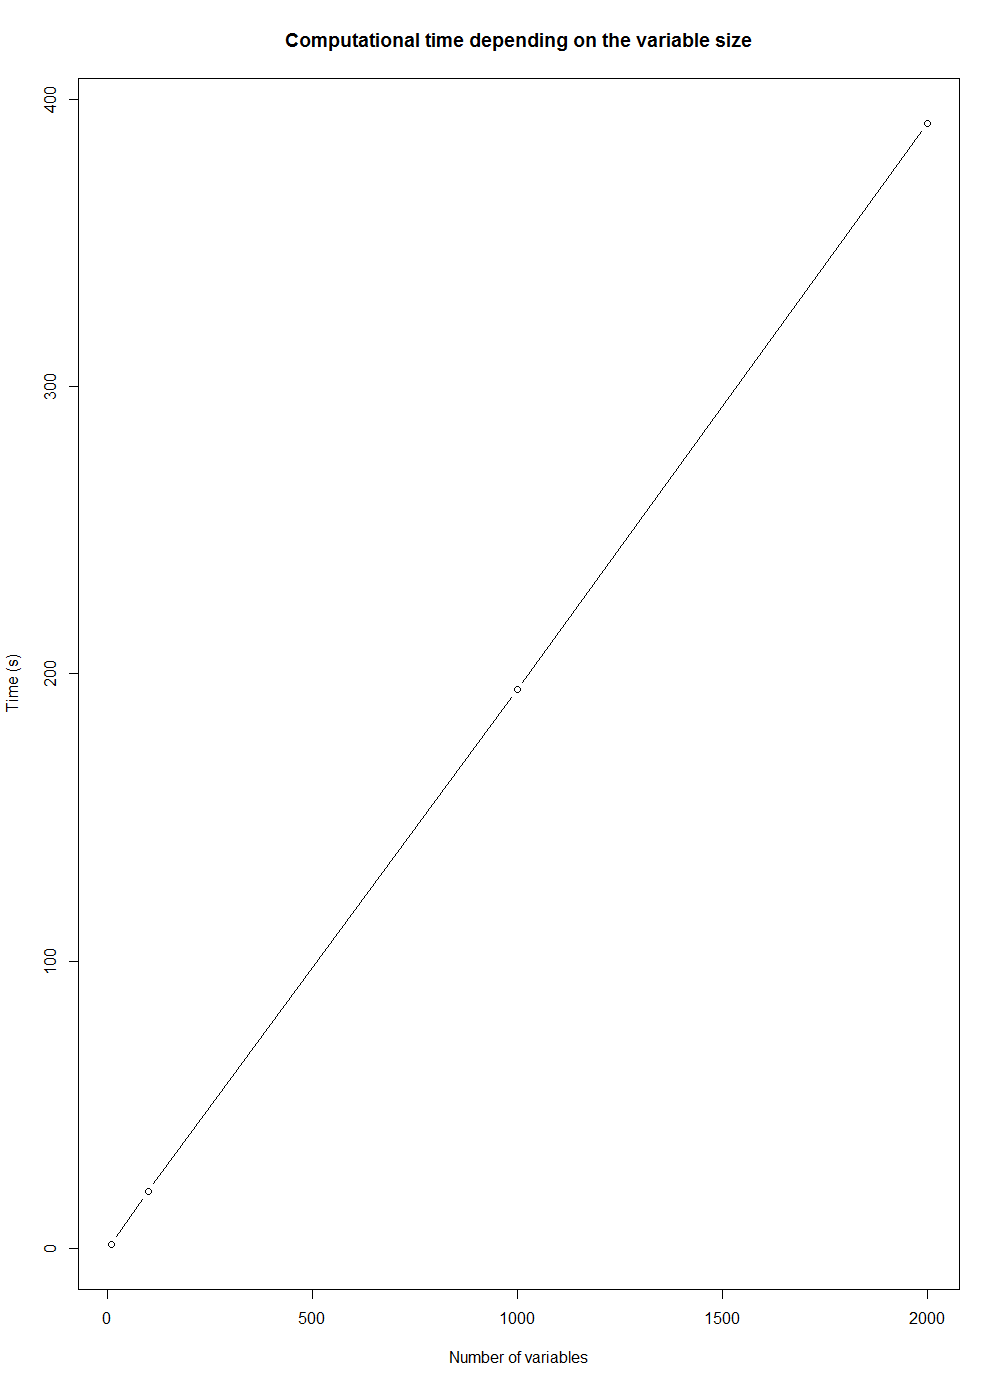
\includegraphics[scale=0.3]{img/VarTime.png}
    \caption{Time consumption evolution in function of number of variables}
    \label{fig:tpsVar}
\end{figure}
\begin{figure}[!]
    \centering
    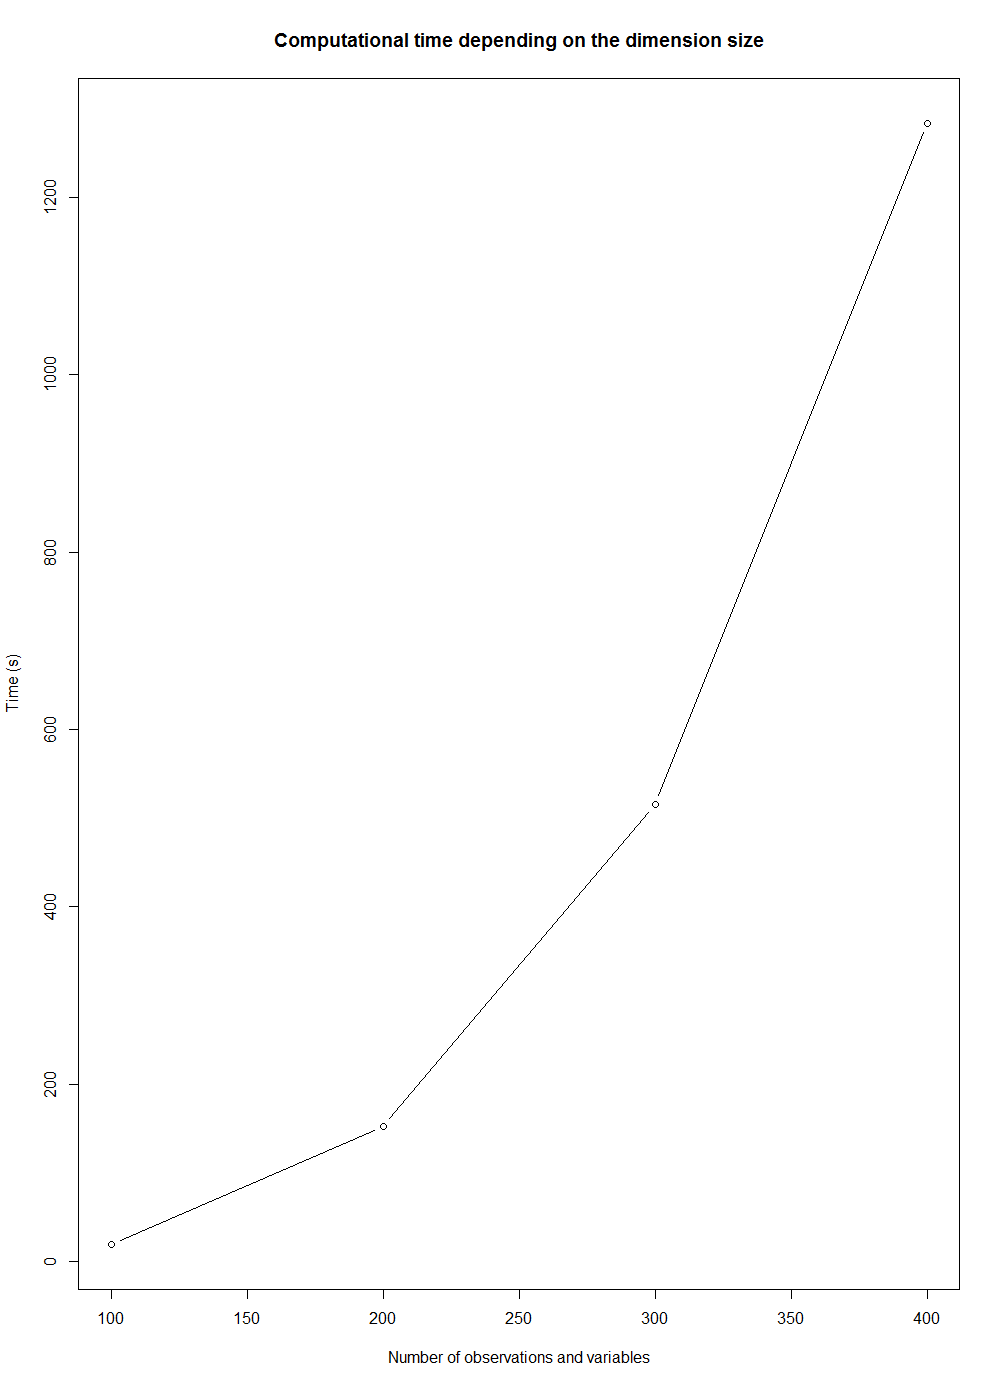
\includegraphics[scale=0.3]{img/bothTime.png}
    \caption{Time consumption evolution in function of number of observations and variables}
    \label{fig:tpsBoth}
\end{figure}


\section{Discussion}

As our results show, the pairwise $\mathcal{L}_{Marg}$ matrix could represent an interesting alternative to distance matrix calculation for mixed type of data.
Indeed, this method is able to mostly find the right number of classes, or at least a close one, for most of the test data sets.
The Top-down clustering algorithm is also able to find a satisfying number of clusters, close to the true one, but not as good as the other method.
Unfortunately, we also showed that although we find a relevant number of clusters, the accuracy is not on point, the Jaccard index struggling to go over 0.5.
Once again an association between the marginal likelihood matrix and a Ward or complete linkage hierarchical clustering outperform the top-down algorithm and even in some cases the Gower distance usage or equating it, i.e: Credit, Dermatology, Zoo data sets.
The lack of accuracy of the top-down clustering algorithm can be explained by the splitting condition, too simplistic, and maybe the theoretical model, lacking sensitivity.
Hence, we believe that by refining the mathematical expressions, adding for instance a prior on the variance for gene expression profiles and adding an informative prior following a Dirichlet distribution for the clinical knowledge, would improve the accuracy.
Some other techniques could be used to obtain a numerical approximation rather than an analytical expression of the likelihood, like MCMC sampling (Gibbs, Metropolis-Hasting).
Furthermore, finding a relevant splitting scheme at each step of this algorithm, relying on the behaviour of the marginal likelihood, would also lead to better results.
Concerning the marginal likelihood matrix, updating such matrix at each new cluster association should also grants to this method better outcomes, but then, as we highlighted it in section~\ref{sec:tps}, the time complexity would go through the roof.
We strongly believe that a Python or Java implementation rather than R, could provide a significant time consumption improvement, and such languages should also allow a more practical object/data manipulation.
Thus, tuning the mathematical model and working on the optimisation of the algorithms could potentially yield to interesting and attractive new methods for cluster investigation.

\section{Conclusion}

Although further refinements are needed to reach applicable methods, we managed to propose an interesting framework for clustering investigation using Bayesian inference.
The lack of accuracy from our implementations prevented us from moving our analyses forward with adenocarcinoma data sets. Without the ability to cluster accurately our data, we preferred to restrict ourselves concerning any interpretation of the clusters. 
Nonetheless, this paper can provide a good basis for future work, we also gave some hints about possible improvement to such model.
The ability of such model to be applied to any practical use makes it attractive and subject to future enhancement, indeed, the probability distribution can be easily tuned to match the needs and efficiency and readability of hierarchical clustering has already been proven over the years.
Several algorithmic approaches were adopted, hence, we proposed three different hierarchical algorithms, written under R, and a simple model comparison tool, all the source code is available.
On a more personal note, working on Bayesian inference was a great learning opportunity, given the popularity and increasing interest for such statistical scheme, and also represented a challenge given the strong mathematical requirements to understand and implement it.
The occasion to freely develop algorithms was also a first, and gave its fair share of programming challenges as well as a personal opening to unexplored fields of computer sciences.
Concerning Japan, my experience here has been a real pleasure, socially as well as culturally, producing unforgettable memories. It truly represents a chance and a great life experience, the once in a lifetime kind, and I hope to come back in this beautiful and welcoming country as soon as possible.

\printbibliography

\end{document}
